\documentclass[authoryear]{elsarticle}
\usepackage{latexsym}
%\usepackage{rotate}
\usepackage{graphics}
\usepackage{amsmath}
\usepackage{amssymb}
\usepackage{comment}
\bibliographystyle{chicago}



\newcommand{\logit}{\mathrm{logit}}
\newcommand{\I}{\mathrm{I}}
\newcommand{\E}{\mathrm{E}}
\newcommand{\p}{\mathrm{P}}
\newcommand{\e}{\mathrm{e}}
\newcommand{\vecm}{\mathrm{vec}}
\newcommand{\kp}{\otimes}
\newcommand{\diag}{\mathrm{diag}}
\newcommand{\cov}{\mathrm{cov}}
\newcommand{\eps}{\epsilon}
\newcommand{\ep}{\varepsilon}
\newcommand{\obdots}{\ddots}    % change this later
\newcommand{\Ex}{{\cal E}}
\newcommand{\rat}{{\frac{c_{ij}}{c_{i,j-1}}}}
\newcommand{\rmu}{m}
\newcommand{\rsig}{\nu}
\newcommand{\fd}{\mu}
\newcommand{\tr}{\mathrm{tr}}
\newcommand{\cor}{\mathrm{cor}}
\newcommand{\bx}[1]{\ensuremath{\overline{#1}|}}
\newcommand{\an}[1]{\ensuremath{a_{\bx{#1}}}}

\newcommand{\bi}{\begin{itemize}}
\newcommand{\ei}{\end{itemize}}

\renewcommand{\i}{\item}
\newcommand{\sr}{\ensuremath{\mathrm{SRISK}}}
\newcommand{\cs}{\ensuremath{\mathrm{CS}}}
\newcommand{\cri}{\ensuremath{\mathrm{Crisis}}}
\newcommand{\var}{\ensuremath{\mathrm{VaR}}}
\newcommand{\covar}{\ensuremath{\mathrm{CoVaR}}}
\newcommand{\med}{\ensuremath{\mathrm{m}}}
\newcommand{\de}{\mathrm{d}}
\renewcommand{\v}{\ensuremath{\mathrm{v}_q}}
\newcommand{\m}{\ensuremath{\mathrm{m}}}
\newcommand{\tvar}{\ensuremath{\mathrm{TVaR}}}



\newcommand{\eref}[1]{(\ref{#1})}
\newcommand{\fref}[1]{Figure \ref{#1}}
\newcommand{\sref}[1]{\S\ref{#1}}
\newcommand{\tref}[1]{Table \ref{#1}}
\newcommand{\aref}[1]{Appendix \ref{#1}}




\newcommand{\cq}{\ , \qquad}
\renewcommand{\P}{\mathrm{P}}
\newcommand{\Q}{\mathrm{Q}}

\newcommand{\Vx}{{\cal V}}
\newcommand{\be}[1]{\begin{equation}\label{#1}}
\newcommand{\ee}{\end{equation}}




\begin{document}

% Title of paper
\title{Systemic risk and contagion effects in Australian financial institutions and sectors}
% List of authors, with corresponding author marked by asterisk
\author{Piet de Jong,  Geoff Loudon and Weihao Choo \\[4pt]
% Author addresses
\textit{Department of Applied Finance and Actuarial Studies\\ Macquarie University, Sydney, NSW 2109.}
\\[2pt]
%E-mail address for correspondence
{piet.dejong@mq.edu.au}}

% Running headers of paper:
\markboth%
% First field is the short list of authors
{De Jong}
% Second field is the short title of the paper
{Systemic risk}

\maketitle

\section{Literature review}

The starting point for the proposed research is the recent literature and the CIFR targeted areas and APRA aims and functions.
This recent literature includes the following
\cite{adrian2011covar},
\cite{acharya2012capital},
\cite{acharya2012measuring}
and \cite{brownlees2010volatility}.   The proposed research aims to extend and apply these techniques particularly in relation to the entities regulated by APRA.   Thus our  broad aim is to develop, implement and bring to bear recent developments in stress testing  on the aims of APRA and the CIFR targeted research areas detailed above.   

\section{Improved  measures of contagion and systematic risk}
\renewcommand{\c}{\ensuremath{\mathrm{CoVaR_q}}}
\renewcommand{\v}{\ensuremath{\mathrm{VaR}_q}}

$\covar_q$ as proposed in \cite{adrian2011covar} is a basis for proposed measures contagion, exposure and systemic risk.   It  suffers from a number of drawbacks:
\bi
\i Couched in terms of $\var_q$ containing the scale of the original measurements.   It is worthwhile to have measures and techniques robust to scale.
\i  Conditioning  on $\var_{0.5}$ is undesirable and relatively intractable.  In our proposal we reference stress with respect  to the unconditional $\var_q$.   This permits a more transparent analysis and estimation. 
\i  Our proposed approach  separates out scale effects and interdependence effects and aims to  relates these separately to external variables including shocks and drivers of systemic risk.   Thus $\var_q$ movements due to scale are disentangled from movements due to codependence with separate driver responses.
\ei

\section{Significance of the project and  policy implications}

Understanding the impact of external shocks and their propagation through   the financial system is vital for managing and remediating systemic risk. Effective regulation is dependent upon the development of a robust and reliable set of appropriate risk measures.  We propose new measures of systemic risk that relate marginal and joint distributions separately to external drivers. This allows for more cogent and coherent stress testing as it includes the estimation of contagion effects, exposure effects and systemic risk across related entities and different financial sectors. Improved stress testing, estimation of risk effects and transmission of shocks through the financial system will make for more cogent prudential policy, prudential margin setting and better identify sources of risk to the financial system.

\newcommand{\q}{\mathrm{Q}}
\section{Percentile sensitivity and contagion}\label{perc}

\subsection{Theorem}  Suppose $x$ is a random vector with marginal distributions\footnote{To economise on notation, write $F_j(x)\equiv F_j(x_j)\equiv F(x_j)$ and similar for other vector functions.} 
$$
F(x)\equiv \{F(x_1),\ldots ,F(x_p)\} \equiv (u_1,\ldots,u_p)\equiv u\ .
$$ 
Further suppose $0\le q\le 1$ is given and  $\q(x)$ is the vector of $q$--quantiles
$$
F\{\q(x)\}=q1=\q(u)\ ,
$$
where $1$ is a vector of $p$ ones. 
Define the stress vector with respect to $x_j$ as\footnote{In \cite{adrian2011covar}  $\Delta CoVar_q\equiv q_{y|x=q_x}-q_y$.  Variable $y$  is generally the ``financial system" and hence considered is the change in the \v\ of the system when institution $x$ stressed, with stress  interpreted as $x=q_x$.  On page 10 of their paper they incorrectly state ``... $CoVaR$ conditions on the event that [an] institution is at its VaR level, which occurs with probability $q$."} 
\be{stress}
\frac{\de\q(x)}{\de x_j} \equiv \q(x|u_j>q) - \q(x)\ ,
\ee
where $\q(x|u_j>q)$ is the vector of $q$--quantiles of $x$ given $u_j>q$.    Then if $\q(x)$  is linear in $q$ 
 then
\be{implicit}
\frac{\de\q(x_i)}{\de\q(x_j)} \equiv \frac{\de\q(x_i)/\de x_j}{\de\q(x_j)/\de x_j} =  
\frac{f_j}{f_i} 
 \frac{q_{ij}}{q(1-q)}\cq q_{ij}=C_{ij}(q+q_{ij},q) - q^2\ ,
\ee
where $f_i$ and $f_j$ are the densities of $x_i$ and $x_j$ evaluated at $\q(x_i)$ and $\q(x_j)$ and  $C_{ij}$ is the copula of $(u_i,u_j)$.   
Further if 
$$
s_{ij}\equiv \frac{q_{ij}}{q(1-q)}\ ,
$$ then  $-1\le s_{ij}\le 1$ with $s_{ij}=\pm 1$ if $x_i$ and $x_j$ are comonotonic and counter monotonic, respectively.  If $x_i$ and $x_j$ are independent then  $s_{ij}=0$. If $u_i$ and $u_j$ are exchangeable  then  $s_{ji}=s_{ij}$.

\subsection{Proof}

By definition
$$
\frac{\de\q(u_i)}{\de u_j} \equiv \q(u_i|u_j>q) -q \equiv q_{ij}\ ,
$$
where  $q_{ij}$ is such that
\be{Qdef}
q =  \frac{\P(u_i\le  q+q_{ij},u_j>q)}{1-q}  = \frac{ q+q_{ij}-C_{ij}(q+q_{ij},q)}{1-q}\ ,
\ee
Rearranging yields the second equation in \eref{implicit}.
Now
 \be{first}
 \frac{\de\q(x_i)}{\de x_j}\equiv \q_{q+q_{ij}}(x_i) - \q(x_i) \approx \q'(x_i)q_{ij}= \frac{q_{ij}}{f_i} \ ,
 \ee
where $'$ denotes differentiation with respect to $q$ and the subscript on $\q$ indicates the revised $q$ for the quantile calculation.  The approximation follows from a first order Taylor expansion and is exact if the quantile is linear in $q$.   Similarly
 \be{second}
 \frac{\de\q(x_j)}{\de x_j}\equiv  \q_{q+q(1-q)}(x_j) - \q(x_j)\approx \frac{q(1-q)}{f_j}\ .
 \ee
 Dividing \eref{first} by \eref{second} yields the first equation in  \eref{implicit} and completes the proof.

\subsection{Discussion}  The critical  result is that sensitivities factor into contributions from the ratios of the marginal densities and quantities calculated from the pairwise copulas.  The via  the implicit  equation for $q_{ij}$ in \eref{implicit}, solved using a  root finding algorithm.
  The quantities $q_{ij}$ are implicitly defined from the pairwise copulas. In summary the ``sensitivity" matrix 
$$
S \equiv \frac{\de Q(x)}{\de Q'(x)}\ ,
$$
where $'$ denotes transposition has ones on the diagonal quantities between $\pm 1$ off the diagonal.   The matrix $S$ is called the sensitivity matrix and displays the sensitivity of the $q$--quantile of  each component of $x$ to  stress in the same or other components.  

Since $f_i$ and $f_j$ are  the densities evaluated at $\q(x_i)$ and $\q(x_j)$  it follows that the ratio $f_i/f_j$ can be replaced by the ratio of the hazards.   This is  useful in cases were it is practical to model the hazard rather than the density.


\subsection{Implementation}

\fref{fig1} displays the empirical copulas calculated from four weekly closing stock prices labelled anz, cba, mcq and  wbc for $n=761$ weeks from 2000 April 12 through to 2014 October 29.  The empirical copulas are calculated by converting each observation to an empirical percentile and plotting the same against each of the other series percentiles.  

\begin{figure}
  \begin{center}
    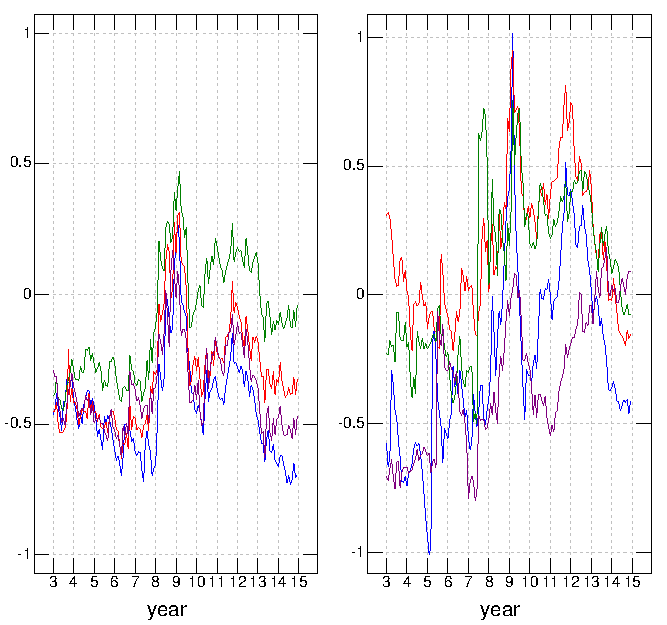
\includegraphics{fig1.pdf}
    \caption{Pairwise copulas of bank stocks  cba, anz, mqg, wbc, and the overall bank index.  Red lines plot sensitivity $s_{ij}$ as a function of $q$.}\label{fig1}
   \end{center}
\end{figure}


To estimate  $q_{ij}$  at a particular $q$, the second equation in \eref{implicit} is iterated\footnote{The second equation in \eref{implicit} is a contraction mapping and hence has a fixed point.} starting from $q_{ij}=0$ where copulas are estimated as 
$$
\hat C_{ij}(u_i,u_j) \equiv \hat\E\{(p_{ik}\le u_i)(p_{jk}\le u_j)\}\ .
$$
Here $\hat\E$ computes the empirical mean over the cases $k=1,\ldots,n$ and $p_{ik}$ and $p_{jk}$ are the empirical percentiles  of case $k$ of $x_i$ and $x_j$, respectively.

\subsection{Generalisations}
\renewcommand{\r}{\mathrm{R}}
Similar results apply when $\Q(x)$ is replaced by  other risk measures such as $\r(x)\equiv\E\{xr(u)\}$ where $r$ is a given function which acts componentwise and $xr(u)$ denotes componentwise multiplication.  For example if $r(u)=mu^{m-1}$ then  $\r(x)=\E\{\max(x^1,\ldots,x^m)\}$ where  $x^1,\ldots,x^m$ are $m$ independent copies of $x$ and the risk measure is the expected worst outcome in $m$ independent trials.

With $\r(x)$, the analogue of \eref{stress} is 
\be{stress2}
\frac{\de\r(x)}{\de x_j} \equiv \r(x|u_j>r_j) - \r(x_j)\cq r_j\equiv\p\{x_j\le\r(x_j)\} \ .
\ee
This differs from \eref{stress}  in that a different risk measure is used and  $r_j$ replaces $q$.   If  the components of $\r(x)$ are linear in the $r_i$ then
\be{implicit2}
\frac{\de\r(x_i)}{\de\r(x_j)} =  
\frac{f_j}{f_i} 
 \frac{q_{ij}}{q(1-q)}\cq q_{ij}=C_{ij}(r_i+q_{ij},r_j) - r_ir_j\ ,
\ee
where $f_i$ and $f_j$ are the $x_i$ and $x_j$ densities at the $r_i$ and $r_i$ quantiles, respectively. 

\section{Systemic risk}
\cite{brownlees2015} describe a model for systemic risk (SRISK) estimated for each financial firm $i$ and each time point $t$.    SRISK of a firm at time $t$ is the expected capital shortfall  it will experience in the period $(t,t+h)$ given a crisis downtown in the market over the same period.    Capital shortfall is defined as the ratio of equity to equity plus debt falling below a certain level $k$.  A crises market is a market return below $c$. 

If expected capital shortfall  is zero then SRISK is zero.   The sum of  SRISK's  across all firms is the total SRISK in the economy and each firm contributes either zero or some proportion to the total SRISK in the economy.    Firms with a high  percentage SRISK (denoted SRISK\%) are systemically important and will be  of major concern to regulators. 




\subsection{Debt and Equity}

Suppose a firm at time $t$ has debt $D_t$ and equity $W_t$.   Then at $t$, $D_t+W_t$ is the total claim on the firm. 
Regulated firms are generally required to hold a proportion $k$ of total claims $k(D_t+W_t)$ as a prudential margin.    If  $k(D_t+W_t)>W_t$ then, prudentially speaking, the firm has capital shortfall   
$$S_t\equiv k(D_t+W_t)-W_t\ .
$$  
Negative capital shortfall indicates positive working capital.

Concerned with predicting capital shortfall $S_{t+h}$ conditional on a systemic event defined as a market decline below a threshold $c$ over the time horizon $(t,t+h)$.  This is similar to \cite{acharya2012wp}.

\subsection{Returns, leverage and capital shortfall}

Consider a single firm with return $r_t$.   This is the percentage change in value over the period  $(t-1,t)$ known as period $t$.   The arithmetic return over the period $(t,t+h)$ is $\nu_t\equiv r_{t+1}+r_{t+2}+\cdots+r_{t+h}$ and is an $h$ period return.  If $h=1$ then  $\nu_t=r_{t+1}$. 

The equity of a firm at time $t+h$ is 
$$
w_{t+h} = (1+\nu_{t})w_t\cq \nu_t\equiv r_{t+1}+\cdots+r_{t+h}\ ,
$$

If the debt of the firm $d_t$  stays constant over the period $(t,t+h)$:   $d_t=d_{t+1}=\cdots=d_{t+h}$  and the capital shortfall i 
\be{cs}
c_{t+h}\equiv  k(d_{t+h}+w_{t+h})-w_{t+h} = k d_{t} - (1-k)(1+\nu_{t})w_t
\ee
 Note  $c_{t+h}$ is a linear in $\nu_t$.

\subsection{Systemic events and systemic risk of a firm}
A systemic event or ``crisis"   occurs in the period $(t,t+h)$ if the market  return $r_{mt}(h)\le c$.   The systemic risk (SRISK)  of  a firm is the expectation of the capital shortfall given  a crisis:
\be{sr}
\mathrm{SRISK}_t\equiv  \E_t\{S_{t+h}|r_{mt}(h)\le c\}  =  [k\ell_t-(1-k)\E_t^c\{r_{t}(h)\}-1]W_t\ .
\ee
where
$$
\mathrm{LRMES}_t \equiv \E^c\{r_{t}(h)\}\equiv \E_t\{r_t(h)|r_{mt}(h)<c\}\ ,
$$
and in terms of this notation:
$$ 
 \mathrm{SRISK}_t = \{k\mathrm{LVG}_t - (1-k)\mathrm{LRMES}_t - 1\}W_t\ .
$$
The condition $D_{t+h}=D_t$ or less strongly $\E_t^c(D_{t+h})=D_t$ indicates the value of debt  does not change if there is a crisis.   

Evaluating the systemic risk in a firm requires the evaluation or estimation of the ``crisis" expectation, also called  the long run marginal expected shortfall (LRMES):

$\mathrm{SRISK}_t$ is a point estimate of capital shortfall in a crisis.   Since $S_t$ is linear in $r_t$ the crisis distribution of $S_t$ is known if the conditional distribution of $r_t(h)|r_{mt}(h)<c$ is known.      
 
\subsection{Vector generalisation} 

Aggregate systemic risk is 
$$
\mathrm{SRISK}_t = \sum_i \mathrm{SRISK}^+_{it}
$$
where $^+$ indicates the positive part of.   
   The proportion of systemic risk in firm $i$ is then
$$
\mathrm{SRISK\%}_{it} = \frac{\mathrm{SRISK}_{it}^+}{\mathrm{SRISK}_{t}}
$$ 

\subsection{Example from vlab}
See \fref{vlab} taken on 15 April 2015 from the website http://vlab.stern.nyu.edu

\begin{figure}[htbp]
\caption{default}\label{vlab}
\begin{center}
%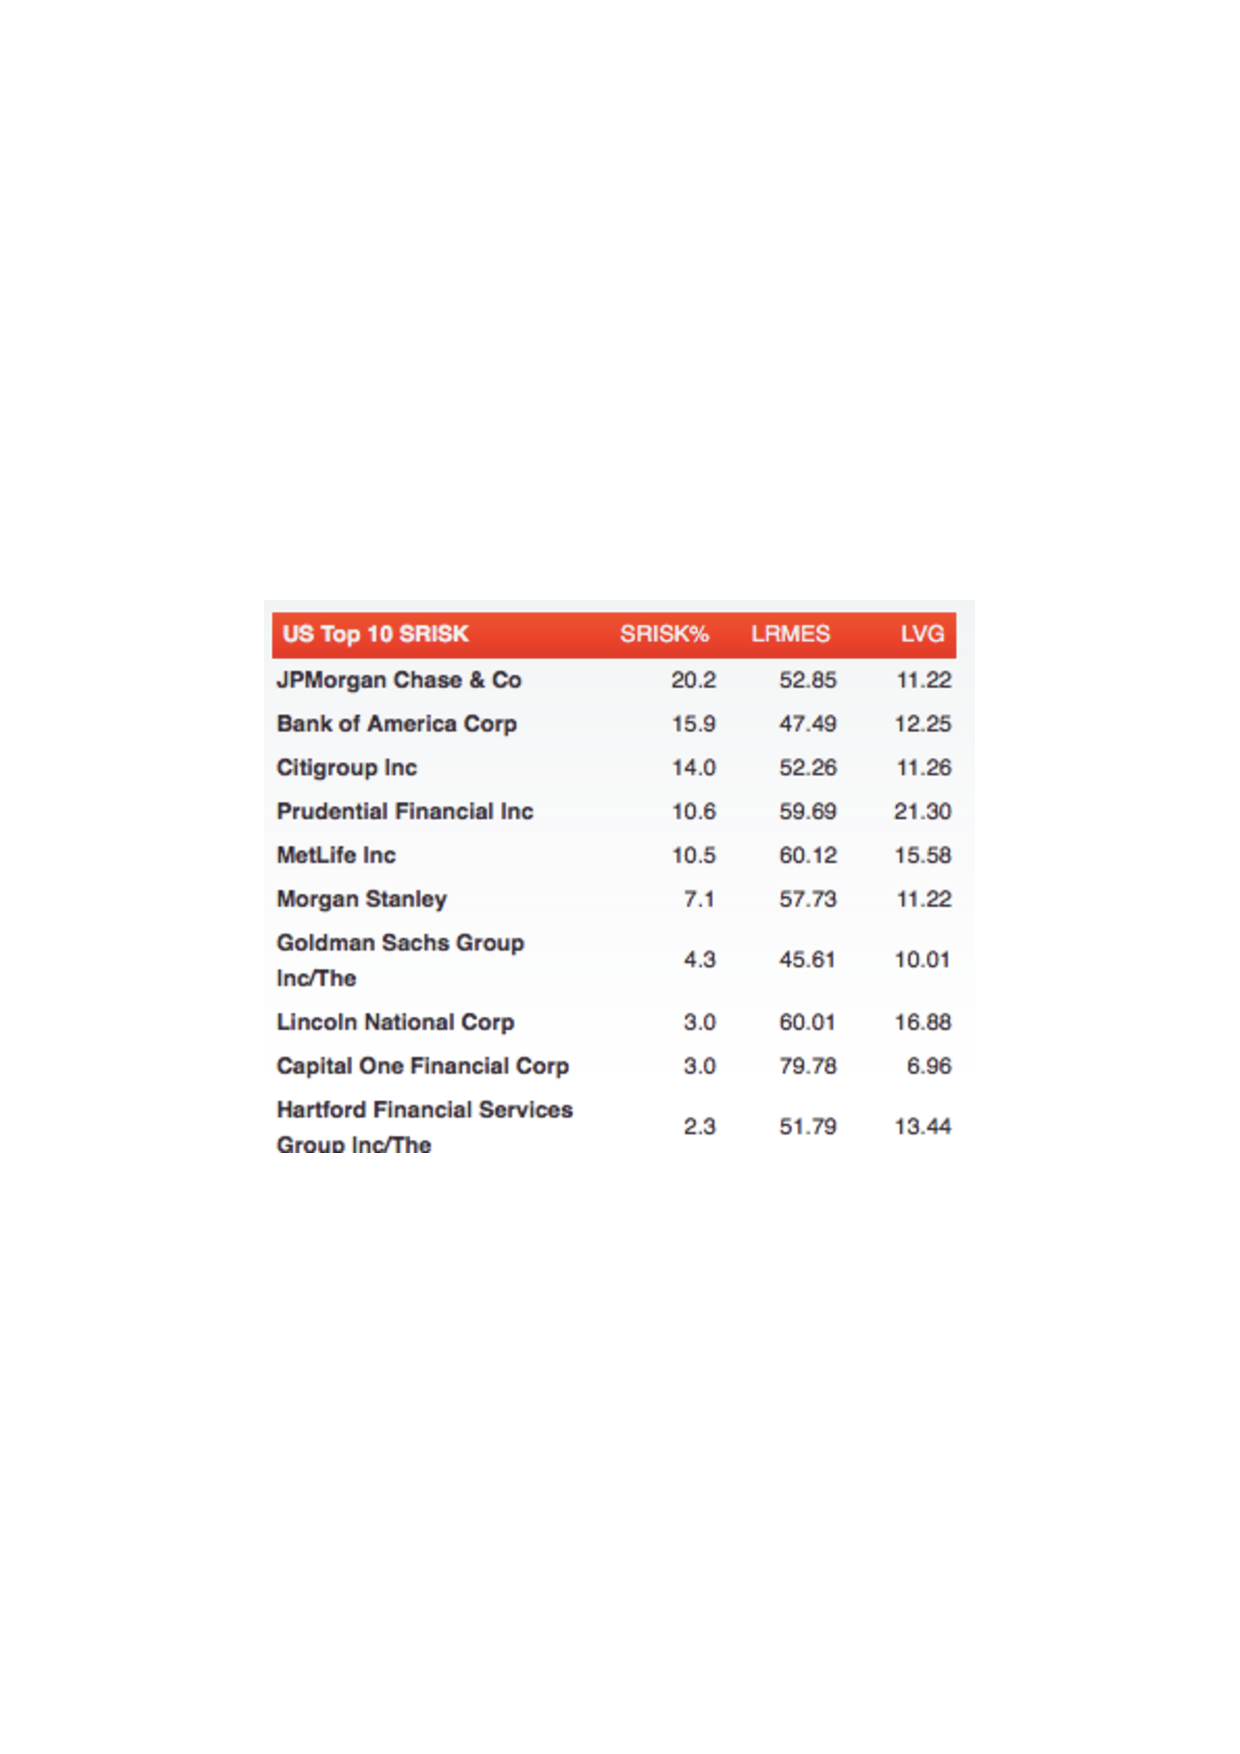
\includegraphics[width=15cm]{vlab.pdf}
\end{center}
\end{figure}

\subsection{Discussion points}

\begin{enumerate}
\item  Above is similar to ``stress tests" regularly applied to financial firms.   However above uses only publicly available information
\item  Above approach is forward looking -- ie distribution of future assets conditional on a systemic event.  Markets look at things forwardly so incorporating forward information.
\item  Should have an appropriate $h$ and $c$ -- not too small etc.
\item  Capital shortfall is natural to use since this generates reduced lending activiity etc.
\item Measuring distress a firm is going to suffer conditional on a systemic event affecting the entire system.   Note this is different from capital shortfall conditional on firm default as with credit models.
\item Not concerned with the probability of joint distress of a large proportion of firms in the financial system.   Here systemic risk is determined by the capital shortfall generated distressed institutions conditional on a systemic event.  Framework takes into account joint dependence among firms, as well as their size and degree of leverage.   Do a small number of large financial institutions pose systemic threats to the entire system?  Tail correlations might fail to do so.
\item  Simplifying assumptions are made to deliver a measure that can be easily computed in practice.    Asset structure is captured in a limited sense.   
\item   Measurement approach can be applied to non financial firms.   However these firms are not highly levereged and are not as vulnerable as financial firms.    Not clear how capital shortfall transmits to rest of economy.   

\end{enumerate}


\subsection{Static econometric model for systemic risk}

An econometric models  links one period returns $r_{it}$  to the  market return $r_{mt}$ enabling  the calculation of 
LRMES and SRISK.   The approach is to assume $(r_{it},r_{mt})$ are zero mean bivariate normal with volatilities $\sigma_{it}$ and $\sigma_{mt}$ and correlation $\rho_t$.  In this case
$$
\E(r_{it}|r_{mt}<c) = \frac{\rho_t\sigma_{it}}{\sigma_{mt}}\E(r_{mt}|r_{mt}<c)  = \rho_t\sigma_{it}\psi\left(\frac{c}{\sigma_{mt}}\right)\cq \psi(x)\equiv\frac{\phi(x)}{\Psi(x)}\ .
$$
Noting $r_{it}(h)=r_{i,t+1}+\cdots+r_{i,t+h}$ and similarly for $r_{mt}(h)$ then 
$$
\E\{r_{it}(h)|r_{mt}(h)<c\}  = \sqrt{h}\rho_t\sigma_{it}\ \psi\left\{\frac{\ln(1+c)}{\sigma_{mt}\sqrt h}\right\}\ .
$$
{\it Let us emphasize that the [last] formula ... has an error which is due to the fact that we are approximating MES using compound returns rather than arithmetic returns.    In particular [the] formula ... has a negative approximation error  and provides more extreme negative LRMES values.}

\subsection{Modelling systemic risk using a dynamic model}

\cite{brownlees2015} use  data on 95 large US financial firms for the period 2000-2012:   daily equity returns and market capitalization from CRSP; quarterly book values for equity and debt from Compustat.   A   Dynamic Conditional Correlation (DCC) model is estimated for  firm and market returns.  Write
\newcommand{\veps}{\varepsilon}
$$
\cov (r_t|t) = V_tR_tV_t'\cq R_t\equiv \cov(\veps_t|t)\cq \veps_t=V_t^{-1}r_t\ ,
$$
where $R_t$ and  $V_t$  are the correlation and diagonal volatility matrix, respectively, at time $t$.   Volatilities in $V_t$  are estimated using univariate threshold GARCH models.  The estimate of $R_t$ corresponds to the correlations in covariance matrix $C_t$ assuming
$$
(C_t - C) = \alpha (C_{t-1}-C)+\beta (\veps_t\veps'_t-C) \cq C\equiv\cov(\veps_t)\ .
$$
where $C$ is the long run covariance matrix.

\cite{brownlees2015} find the above systemic risk measure  a)  successfully identifies systemically risky firms during the GFC;
b)  predicts capital injections by Fed Reserve; and c) aggregate systemic risk provides early warning of declines in industrial production and higher unemployment.

Thus the model  estimates the beta of a firm equity on a broad market index.
A bivariate volatility model is estimated for the return on the broad market and the equity return of each firm. This model allows volatilities and correlations to evolve.    The estimated process is used to simulate the probability of severely negative outcomes over an extended period. Assuming that firms can only operate if capital is a non--trivial proportion of their total liabilities, SRISK is defined as the capital that would be needed to achieve a market cap that is 8\% of the book value of assets in the event of a crisis. The input to SRISK is size, leverage and risk. Each is important and a firm that wants to reduce its SRISK, can operate on any of these characteristics. A crisis is taken to be a 40\% drop in global equity values over six months. SRISK is computed weekly for firms from about 70 countries and published on the internet at http://vlab.stern.nyu.edu.  In extending this analysis to international markets, the model is naturally generalized to a multivariate volatility model. The data are considered to be the equity return on one firm, the equity return on a global index of equity returns, and perhaps some lags. The use of daily data for assets that are priced in different time zones means that closing prices are not measured at the same time and consequently there may be some important effect from lagged factor returns.

\subsection{Systemic risk based on probabilities}

If $d_t$ and $w_t$ are the debt and equity of a firm at time $t$ then the capital shortfall at time $t$ is 
$$
(1-k) d_t  - k w_t
$$
Basel II assumes $1-k=0.08$ implying there is  positive  capital shortfall if 
$
 0.08 d_t>0.92 w_t
$
or  leverage $d_t/w_t>11.5$ or the log--leverage is greater than $\ln(11.5)=2.44$.  
	
Given the debt and equity, the capital shortfall at time $t$ is zero if 
$$
\frac{k_t}{1-k_t} = \frac{d_t}{w_t}\cq k_t= \frac{d_t/w_t}{1+d_t/w_t} = \frac{d_t}{d_t+w_t}
$$
where $0\le k_t\le 1$  is thought of as a risk index and $k_t/(1-k_t)$ is the leverage or risk odds.   


Now consider the situation at time  $t+h$ where $h>0$, 
$$
 k_{t+h}\equiv\frac{d_{t+h}}{d_{t+h}+w_{t+h}} =  \frac{d_t}{d_t+\e^{\nu_{t+h}}w_t}
$$ 
where it is assumed $d_{t+h}=d_t$ and $\nu_{t+h}$ is the $h$ period return over $(t,t+h)$.  The   logit risk/log leverage is
$$
\ell_{t+h}\equiv\ln \frac{k_{t+h}}{1-k_{t+h}} = \ln \frac{d_{t+h}}{w_{t+h}} = \ln d_t - \ln w_t - \nu_{t+h} = \ell_t -\nu_{t+h} \ .
$$
Hence a large positive return $\nu_{t+h}$ implies a lower  risk.  As the logit risk/log leverage  increases to 2.44 the firm approaches the Basel II threshold.

If there are a number of  firms $i$ then $\ell_t$ and $\nu_{t+h}$ are  vectors with components $\ell_{it}$ and $\nu_{it}$, respectively, and in vector terms, $\ell_{t+h}=\ell_t - \nu_{t+h}$.   The aggregate risk is $1'\ell_{t+h}$.


\subsection{Systemic risk}

Systemic risk is defined as the log--leverage in the system as a whole:   that is  aggregate all debt and equity and compute, as above, the log--leverage $\ell_t^+$.    Then
$$
\ell^+_{t+h} = \ln \frac{d^+_t}{w^+_t}-\nu^+_{t+h} =  \ln \sum_i\alpha_{it}\frac{ d_{it}}{ w_{it}} -\nu^+_{t+h}= \ln \Ex_w(\e^{\ell_{it}})-\nu^+_{t+h} \cq \alpha_{it}\equiv\frac{w_{it}}{ w^+_t}\ .
$$
where $\nu_{t+h}^+$ is the aggregate return
$$
\ln \frac{1'w_{t+h}}{1'w_t} = \ln\Ex_w(\nu_{it})
$$
Differentiating with respect to $\ell_{i,t+h}$ yields
$$
\frac{\de \ell^+_{t+h}}{\de \ell_{i,t+h}} = \frac{\alpha_{it}\e^{\ell_{it}}}{\sum_i\alpha_{it}\e^{\ell_{it}}} \frac{\de\nu_{i,t+h}}{\de \ell_{i,t+h}}=\frac{w_{it}\e^{\ell_{it}}}{\sum_iw_{it}\e^{\ell_{it}}}
=\frac{d_{it}}{\sum_id_{it}}=\frac{d_{it}}{d_t^+}\ ,
$$
implying the percentage change in overall forecast leverage respect to a percentage change of the forecast leverage of  firm $i$ is proportional to the proportion of debt in firm $i$.   Further 
$$
\ell^+_{t+h} = \ln \Ex_w(\e^{\ell_{it}})-\nu^+_{t+h} \approx \Ex_d(\ell_{it})-\Ex_d(\nu_{i,t+h})\
$$
Thus the contribution of firm $i$ to the systemic risk is 


\subsection{Comparing default probabilities}

Suppose $\ell_{it}$ and $\ell_{t}$ are the risk for firm $i$ and the combination of firms.   Then the excess risk in firm $i$ is
$$
\ell_{it}-\ell_t = \ln \frac{d_{it}}{d_t} - \ln \frac{w_{it}}{w_t} + (\nu_t-\nu_{it})\ .
$$
Thus if firm $i$ has the the same leverage as the average leverage then the excess risk is the underperformance over the time interval $(t,t+h)$. 

Note

and hence can define
$$
x
$$


\subsection{Systemic risk}

The total leverage in the system is

a value weighted average of the individual leverages.   The $k_t$ for  capital shortfall for the system as a whole can be
produced from this total leverage.   The logit $\ell_t$ of $k_t$ then yields a risk index for the system as a whole.  Note
$$
\ell_t \equiv \ln \frac{d_{t+h}}{w_{t+h}}=-\nu_t+\ln \sum_i\alpha_{it}\frac{ d_{it}}{ w_{it}}\ne \sum_i \ell_{it}
$$

Can look at
$$
\ell_{it}-\ell_t  = \ln d_{it}-\ln d_t - (\ln w_{it}-\ln w_t) - (\nu_{it}-\nu_t)
$$

Suppose there are a number of firms and define
$$
d_t=\sum_i d_{it}\cq w_t=\sum_i w_{it} \cq  \frac{\ell_{it}}{\ell_t}
$$



The log--odds can be related to other variables.  In many cases the capital injection required is negative indicating capital can be withdrawn from the company without it breaching prudential standards.




\subsection{GARCH-DDC simulation}

We can consider the distribution of the projected log--leverage (pll) conditional on other variables including the market return
$$
\E(\ell_t|\nu_{mt}\le c)  = \ln d_t -\ln w_t -\E(\nu_t|\nu_{mt}\le c)\ .
$$
Alternatively we can consider the  $\alpha$--percentiles of $\ell_t$ denoted $\ell^\alpha_t$ such that
$
\alpha=\P(\ell_t\le \ell_t^\alpha)
$.  Note
$$
\ell_t^\alpha = \ln d_t -\ln w_t -\nu_t^\alpha = \ln \frac{d_t}{w_t}-\nu_t^\alpha\  .
$$

The GARCH-DCC setup delivers forecast or simulated values of $r^s_{t}(h)$, $s=1,\ldots, S$  for each  $t$.      Assume the simulated values are ordered in terms of increasing market returns $r^s_{mt}(h)$ and arranged in an $2\times S$ matrix $C_t$ where  the bottom row is the simulated market return.

This computation is complicated by two things:
\begin{enumerate}
\item  Dividends my be paid  in the period $(t, t+h)$ serving to reduce equity.  Typically at most one dividend  is payable which can be accumulated to  $t+h$ and used to increase equity.   That is for purposes of  assessing model accuracy $w_{t+h}$ is increased by proportion $1+f_{t'}(1+r_{t'})^{t+h-t'}$ where $t\le t'<t+h$ is  ex--dividend date and $f_t$ is the dividend yield.
\item  Debt may change over the period.
\end{enumerate}

In terms of $C_t$ the SRISK measure of \cite{brownlees2015} is the average, along each row of the prefixes.  For example,  the average in row $i$ of the  first $s$ entries is the systemic risk of firm $i$ at time $t$ conditional on  $r_{mt}(h)\le F_{mt}^{-}(s/S)$ where  $F_{mt}$ is the empirical distribution of the  $r^s_{mt}(h)$, $s=1,\ldots,S$.

A default or breach of prudential margins occurs if $c_{it}^s>0$.  The probability of a default if $r_{mt}(h)\le F_{mt}^{-}(v)$ is estimated as 
$$
\hat p_{it}=\frac{\sum_{s=1}^{[vS]}I(c^s_{it}>0)}{[vS]}\ ,
$$
where $v$ is given, for example $v=0.1$.
Joint probabilities of default are estimated similarly: the joint probability of a subset $B$ of firms  breaching their margins is 
estimated as
$$
\hat p_{Bt} = \frac{\sum_{s=1}^{[vS]}\prod_{i\in B} I(c^s_{it}>0)}{[vS]}\ .
$$
These probabilities generally decline with $v$: that is as the market downturn becomes less extreme.

Instead of asking what is the probability of a default (ie breach of prudential regulation) it is meaningful to consider what would $k$ have to be in order for it to be in default at time $t+h$.    Writing this value as
$$
k_t d_t - (1-k_t)\{1+r_t(h)\}w_t = 0 \qquad \implies \qquad k_t=\frac{1}{1+d_t/[\{1+r_t(h)\}w_t]}
$$
This equation can be computed given $r_t(h)$ and hence for every simulated value to arrive at $k_t^s$.    If $d_t\equiv0$ then $k_t=1$ indicating  a healthy state of affairs.  If $d_t/w_t$ is large then $k_t\approx 0$.    Hence as $k_t$ drops there is more danger. 



Furthermore
$$
\ln k_t = -\ln \left[1+\{1+r_t(h)\}^{-1}\frac{d_t}{w_t}\right]\approx -\{1+r_t(h)\}^{-1}\frac{d_t}{w_t}\approx -\e^{-r_t(h)}\frac{d_t}{w_t}
$$
$$
\kappa_t \equiv \ln(-\ln k_t) \approx  \ln (d_t) - \ln (w_t) - r_t(h)
$$
A large value for $\kappa_t$ indicates 


To study the time series and cross sectional behaviour of $\hat p_{it}$, it is useful to define the  normal scores 
$$
z_{it} \equiv \Phi^-(\hat p_{it})\cq i=1,\ldots, n\cq t=1,\ldots, T\ .
$$
Defining  $z_t\equiv (z_{1t},\ldots,z_{nt})'$ then a firm is systemically important if it is highly collinear with the other scores. 

An entropy based measure of systemic risk is
$$
H_t = -\E(\ln p_{Bt})\equiv -\sum_B p_{Bt}\ln p_{Bt}\ .
$$

Systemically important firms are those which, when in default, are highly likely to be associated with a joint default.
joint probability of matrix is then 
$$
  P_t\equiv \frac{1}{S} I_tI_t'\cq  I_t = I(\rho^s_{it}>0)
$$


 can define the probability of a firm going in default as
$$
\hat p_{it}\equiv \frac{\sum_{s=1}^SI(\rho_{it}^s>0)}{S}
$$ 
In terms of this notation the probability of all firms going bankrupt and non



\subsection{Time--varying copula model}

Suppose $\delta\ge 1$ and the rotated Gumbel copula modelling lower tail dependence:
$$
C_\delta(u,v) = u+v-1+\e^{-[\{-\ln(1-u)\}^{\delta}+\{-\ln(1-v)\}^{\delta}]^{1/\delta}}
$$
Further suppose a sequence
$$
\delta_{t+1} = 1+\left(\omega + \alpha \frac{\sum_{s=0}^{m-1}|u_{t-s}-v_{t-s}|}{m}+ \beta\delta_t\right)^2\ .
$$
Note $\delta_t$ is always greater than 1.  \cite{patton2006modelling} has more details.   The model is fitted by estimating marginal models first and then by maximizing the copula likelihood using the fitted uniform marginals.

\subsection{Data  used in \cite{brownlees2015} }

\begin{itemize}
\item Large US financial firms (ie capitalization greater than 5bln US)
\item Jan 3, 2000 through to Dec 31, 2012:  not all companies continuously traded
\item Daily returns and market capitalization from CRSP
\item Quaterly book value of equity and debt from COMPUSTAT.
\item SIC codes used to segment firms into 4 industry groups (Depositries (29), Broker Dealers (10), Insurance (34) and Others (22))
\end{itemize}

SRISK is computed with the parameters $k=0.08$, $c=-0.1$, $h=22$ (a month).  SRISK computed at end of each month using all available data at that data, therefore no look ahead bias.  

LRMES computed with the GARCH-DCC model for each firm.   Uses all available data starting from Jan 3, 2000 to end of each month.


\subsection{Older stuff}
   
$$
\E^c(r_{it}) \equiv \E(r_{it}|u_{mt}\le c^*)\cq c^*=\E\{(r_{mt}\le c)\}\ ,
$$
where $u_{mt}$ is the percentile of $r_{mt}$.
Given a joint distribution for $(r_{it},r_{mt})$ the distribution is simulated and
\be{sim}
\E^c(r_{it}) \approx \frac{\hat \E\{(r_{mt}\leq c)r_{it}\}}{\hat \E\{(r_{mt}\leq c)\}}= \frac{\hat\E\{(u_{mt}\leq c^*)F^-_{it}(u_{it})\}}{c^*}\ ,
\ee
where the $r$ values in the middle expressions denote simulated values and $\hat\E$, averages over the simulated values.   The $u_{it}$ and $u_{mt}$ are the percentiles of $r_{it}$ and $r_{mt}$, respectively.

The right hand expression in \eref{sim}  suggests using a copula to model the joint distributions $(r_{it},r_{mt})$.  Simulate $(u_{it},u_{mt})$, from the copula, discarding pairs with $u_{mt}>c^*$.   For each accepted $(u_{it},u_{mt})$  determine the actual return using the respective marginal distributions.   Issues to be addressed are:
\bi
\i Are the marginal distributions time invariant?  Could have situation where the marginal distribution evolves over time and/or is state dependent
\i Is the copula time invariant?   Could have situation where the copula is state dependent.    
\ei


The first step here is to examine the marginal distributions of the returns and the empirical copula of returns.



{\bf Comment.}  With the DCC model both volatilities and correlations have a time dependent structure.  These are modelled separately.
An alternative approach is where ...



{\bf \cite{engle2014dynamic}} describes a new approach to estimating time varying regression coefficients.   The approach is called Dynamic Conditional Beta (DCB).   Consider $(y_t,x_t)$ where  $y_t$  and $x_t$ are vectors.  Interested in $\E_t(y_t|x_t)$.   This is expression  may be linear in $x_t$ and depending on the past information set.  Write
\newcommand{\F}{{\cal F}}
$$
(y_t,x_t)|\F_{t-1} \sim N(\mu_t,H_t) \implies y_t|x_t,\F_{t-1}\sim N\{\mu_{yt}+B_t(x_t-\mu_{xt}), C_{yy,t}\}
$$
where
$$
B_t= H_{yx,t}H^-_{xx,t}\cq  C_{yy,t}= H_{yy,t}-B_tH_{xx,t}B'_t\ .
$$
These expressions depend on the time varying covariance matrix $H_t$.    For implementation we need a model for $\mu_t$ and $H_t$.




\section{TARCH modelling}

The standard approach to the joint modelling of returns is where volatility adjusted returns are modelled, for each security, as
\newcommand{\vareps}{\varepsilon}
\be{mean.model}
r_{t}=\mu+\sigma_t\eps_t\cq \eps_t\sim (0,1)\cq  \eps^-_t\equiv(\eps_t<0)=(r_t<\mu)\ ,
\ee
%frac{r_{it} - \mu_i}{\sigma_{it}} = \rho_{it}\eps_{mt} + \sqrt{1-\rho_{it}^2}\vareps_{it}
Further
\be{vol}
\sigma_{t+1}^2 = \omega+ (\alpha+\gamma\eps^-_t) (r_t-\mu)^2 + \beta\sigma^2_t=\omega+ \sigma^2_t\{(\alpha+\gamma \eps^-_t)\eps_{t}^2 + \beta\}\\ .
\ee
Hence the response in the variance to $\eps_t^2$  is increased by $\gamma$   if $\eps_{t}<0$ compared to the response if $\eps_t>0$.  This is a simple threshold GARCH model:  called TARCH.   

The simple TARCH model \eref{mean.model} and \eref{vol} is generalised by replacing $r_t-\mu$ by a time series model possibly including explanatory variables.   Further $\omega$ can be replaced by $x_t'\delta$ where $x_t$ is a vector of explanatory variables, while extra lags can be introduced on the right hand side of \eref{vol}.  

 Taking expectations of both sides of \eref{vol} yields
 $$
\sigma_{t+1}^2 = \omega+ \left\{\alpha+\beta+\gamma \E(\eps^-_t\eps_{t}^2)\right\}\sigma_t^2\ .
 $$
For a long run stationary solution 
$$
\sigma^2 = \frac{\omega }{1-\alpha-\beta-\gamma\E(\eps^-_t\eps_t^2)}\cq \E(\eps^-_t\eps_t^2)=p\E(\eps_t^2|\eps_t<0)+(1-p)\E(\eps_t^2|\eps_t\ge 0)\\ .
$$
where $p\equiv\E(\eps_t^-)$.  For the symmetric case, $p=1/2$ and  $\E(\eps_t^2|\eps_t<0)=1$ implying $\E(\eps^-_t\eps_t^2)=1$ and
$
\omega=(1-\alpha-\beta-\gamma)\sigma^2
$.  With the zeta transform  $\sigma^2=1$ and hence the sum of the coefficients is 1.

Alternatively
$$
\E(\eps^-_t\eps_t^2) = p +\rho\sqrt{p(1-p)} = p\left(1+\rho\sqrt{\frac{1-p}{p}}\right)\ ,
$$
where $\rho$ is the correlation between $\eps_t^-$ and $\eps_t^2$.   For a symmetric distribution this reduces to $(1+\rho)/2$. 

The above setup holds for each security $i$ including the market, assumed to have index $i=m$.   The correlation between securities can also be modelled.   This is achieved by modelling the correlation of each security with the market, denoted $\rho_{it}$ or assuming the correlation matrix of the stack of the $\eps_t$, denoted $\eps_t$  are generated from a positive definite matrix $Q_t$ say where \citep{engle2002dynamic}
$$
Q_{t+1} = (1-\alpha-\beta) S + \alpha \eps_t\eps_t' + \beta Q_t\ ,
$$
where $\eps_t$ is the vector of $\eps_{it}$, including that of the market.

 \section{TARCH modelling applied to zeta scores}
 
 In this case $\omega_i\approx 0$, $\alpha_i$ and $\beta_i$ is generally positive and significant, while $\gamma_i$ is positive and marginally significant.  This suggests in these cases
 $$
 \zeta_{it}=\sigma_{it}\eps_{it}\cq \sigma_{i,t+1}^2= \{\alpha_i + \gamma_i(\zeta_{it}<0)\}\zeta_{it}^2+\beta_i\sigma^2_{it} 
 $$
 Thus negative $\zeta_{it}$ tend to increase volatility while positive $\zeta_{it}$ have no effect on volatility.  The persistence is 
 $$
1+\alpha_i+\frac{\gamma_i}{2}+\beta_i
 $$
 assuming $\E\{(\zeta_i<0)\}=1/2$.   

\section{Lee--Carter modelling of financial variables}

Suppose $r_t$ is a vector of rate of returns with mean vector $\mu$.   Further suppose the returns are standardised so that over time each has mean zero and standard deviation 1.  Then write
$$
\frac{r_{it}-m_i}{s_i}=\beta_i\kappa_t+ \psi_i\eps_{it}\cq \kappa_t= \mu+\sigma_t\eps_t\cq  \eps_t,\eps_{it}\sim N(0,1)\ ,
$$
where $\kappa_t$ is normalised so that $\kappa_1=\overline r_1$ and $\kappa_n=\overline r_n$ and
$$
\sigma^2_{t+1} = \alpha_0+\alpha_1(\kappa_{t}-\mu)^2+ \beta_0 \sigma_t^2\ .
$$
Under the model the variance at time $t$ of the standardised $r_{it}$ is 
$\beta_i^2 \sigma^2_t + \psi^2_i$ while the covariance between $r_{it}$ and $r_{jt}$ is  $\beta_i\sigma^2_t\beta_j$.
Hence the squared correlation between $r_{it}$ and $r_{jt}$ is
$$
\frac{(\beta_i\sigma^2_t\beta_j)^2}{(\beta_i^2 \sigma^2_t + \psi^2_i)(\beta_j^2 \sigma^2_t + \psi^2_j)} = \left\{\left(1+\frac{\psi^2_i}{\beta_i^2\sigma_t^2}\right)\left(1+\frac{\psi^2_j}{\beta_i^2\sigma_t^2}\right)\right\}^{-1}
$$
As $\sigma_t$ becomes large the correlation approaches 1. 

\section{Understanding of model}
\bi
\i  The observed distribution of $r_{mt}$ outcomes is a reasonable reflection of the (unconditional) marginal distribution at each $t$.
\i  Hence the $u_{mt}\equiv \P(r_{mt})$ are reasonable uniforms on the basis of the unconditional marginals
\i  In the standard analysis we use a model describing the conditional distribution at each $t$
\i  To what extent is $u_{mt}$ the conditional uniform i.e. uniforms calculated from the conditional distribution?  Do we need these.  Note that $r_{mt}$ can be viewed unconditionally or conditionally.   i.e. the across time distribution of the $r_{mt}$ will be close the unconditional whereas $r_{mt}$ itself is chosen conditionally if we employ a time series model.     
\i  So it appears the computed $u_{mt}$ can be regarded as unconditional.  (just like $r_{mt}$).    However they can also regarded as generated conditionally.  Ditto for $\zeta_{mt}$ etc.
\i  So suppose we have estimate $\sigma_{mt}$ using a garch model based on either the $r_{mt}$, $\logit \P(r_{mt})$ or $\zeta_{mt}$.   For the latter this is the conditional variance of $\zeta_{mt}$ i.e.
$$
\zeta_{mt}|t-1 \sim N(0,\sigma^2_{mt})
$$
\i So at each future $t$ (forecast or smoothed), given $\sigma_{mt}$  we draw $r_{mt}$ or $\zeta_{mt}$, compute $\P(r_{mt})$ or $\Phi(\zeta_{mt})$.  The former is with respect to the whole distributions whereas the latter is with respect to the normal.
\ei 

\section{ARCH specification}
   A GARCH(1,1) model stated in terms of noise $\eps_t\sim(0,1)$ and time varying volatility $\sigma_t$:
$$
r_t= \mu + \sigma_t\eps_t\cq \sigma^2_{t+1} = \alpha_0+\alpha_1(r_{t}-\mu)^2+ \beta_0 \sigma_t^2\cq \eps_t\sim N(0,1)\ .
$$
Here $\mu$ is the average return, assumed independent of time.

Instead of using  actual returns we can consider the zeta transform $\zeta_t=(\Phi^-\circ \P)(r_t-\mu)$
with 
\begin{equation}\label{garch}
\zeta_t=  \sigma_t\eps_t\cq (\sigma^2_{t+1}-1) = \alpha (\sigma^2_{t}-1) + \beta(\zeta_t^2-1)\cq \eps_t\sim N(0,1)\ .
\end{equation}
The second equation can be written as
$$
\sigma^2_{t+1} = (1-\alpha-\beta) +  \alpha \sigma^2_{t} + \beta \zeta_t^2\ .
$$

Given the fit, \eref{garch} is simulated forward from $t=n$ to yield $\zeta_{n+1},\zeta_{n+2},\ldots$ and in turn
$$
\hat r_{t}=\mu+(\P^-\circ \Phi)(\zeta_{t})\cq t=n+1,n+2,\ldots\ .
$$
The inverse $\P^-$ is  with respect to the empirical distribution, or some modified version of the same  (a stressed version?)

Now take the $u_{mt} = \Phi(\zeta_t)$ and the copulas $C(u_{it},u_{mt})$.   The copula can be the empirical copula or some smoothed version of the same.   Then 
$$
\hat r_{it} = \mu_i + \P^-(u_{it})\cq u_{it}\sim C(u_{it}|u_{mt}) \cq t=n+1,n+2,\ldots\ .
$$
Again, $\P^-$ is with respect to the past distribution of returns $r_{it}$ or some modified version of the same.  With the PG model the $\zeta_{it}$ are chosen given $\zeta_t$ and hence the relation becomes
$$
\hat r_{it} = \mu_i + (\P^-\circ\Phi)(\zeta_{it})\cq \zeta_{it}\sim \mathrm{PG}(\zeta_{it}|\zeta_{mt}) \cq t=n+1,n+2,\ldots\ .
$$
If returns are jointly normal this model reduces to the usual normal modelling.

In terms of this setup:
\bi
\i Future market returns are generated in terms of an ARCH model stated in terms of the zeta transform
\i Relationships (i.e. systemic risk) inherent in other returns are stated in terms of a PG copula
\i Stressing is achieved in terms of stressing $\P_m$.
\ei

suggesting that in an unconstrained fit the coefficients should add to 1.
$$
r_{mt}=(F_m^-\circ\Phi)(\sigma_t\eps_t)
$$
Since $\E(z_t^2)=1$ and $\alpha<1$, then in the long run $\sigma^2_t\rightarrow 1$.   If $z_t$ is in either tail and hence $z_t^2$ is far from  1 then $\sigma^2_{t+1}$ is much bigger than 1 and $z_{t+1}$ will be in the tail.   Then
\be{forward}
r_{it}=F_i^-(u_{it})\cq u_{it}\sim C\{u_{it}|\Phi(z_t)\}
\ee
Thus volatility clustering occurs since $z_t$ in one or tail, drives, via the copula, both $r_{it}$ and $r_{jt}$ into the tail.      

Steps in fitting:
\begin{enumerate}
\i  An ARCH model is fit to the market return $z_t=(\Phi^-\circ F_m)(r_{mt})$ where $F_m$ is the empirical distribution of the market rates
\i  The $z_t$ is simulated forward from time $t=n$ using the ARCH model. 
\i  Retain only those forward simulations such that the cumulative drop $\prod_{t=n+1}^N\{1+(F_m^-\circ \Phi)(z_t)\}$ is less than the crisis drop.
\i  For each forward simulated value, chose $r_{it}$ using the conditional copula and simulation smoothing
\i Calculate the capital shortfall for firm $i$.
\end{enumerate}

   
The rationale is that  $(y_{t}-\mu)^2$ is the latest available estimate of the variance at time $t$ and this latest   estimate is combined with the  ``permanent" component $\sigma^2_{t}$.   Constraints  are required on $a_0$, $a_1$ and $b_1$ to ensure $\sigma_t$ stays positive and finite.  If  $a_1=b_1=0$ then $y_t$ is noise with mean $\mu$. 

In our case $y_t=z_t$ is standard normal so we can drop $\mu$ to get
$$
z_t=  \sigma_t\eps_t\cq \sigma^2_{t+1} = a_0+a_1 \sigma^2_{t} + b_1z_t^2\ .
$$ 


Fitting GARCH models with R.  The  command $garch(y,c(1,1))$ fits  model $garch$ to $y$.  The $garch$ command requires $library(tseries)$. 

The quantity $a_0/(1-a_1-b_1)$ is the long run average $\sigma^2_t$ since it is the constant solution to the right hand side equation \eref{garch}, if  $(y_t-\mu)^2$ is replaced by its expectation.    We want the long run average to be 1 implying
$
a_0=1-a_1-b_1
$ and hence
$$
z_t=  \sigma_t\eps_t\cq \sigma^2_{t+1} = a_0+a_1 \sigma^2_{t} + (1-a_0-a_1)z_t^2\ .
$$
$$
z_t=  \sigma_t\eps_t\cq (\sigma^2_{t+1}-1) = a_1 (\sigma^2_{t}-1) + (1-a_0-a_1)(z_t^2-1)\ .
$$



 \fref{fig7} displays output from fitting a GARCH model to the daily percentage returns of the FTSE index plotted in \fref{fig6}.   In this fit  $\mu$ is set to the sample mean return, $\hat a_1=0.045$ indicates moderate autocorrelation in the standard deviation while $\hat b_1= 0.942$ indicates high reaction to the latest volatility $(y_t-\mu)^2$.  The long run average standard deviation is $\sqrt{0.009/(1-0.045-0.942)}=0.825$, marginally above the empirical standard deviation of 0.796.   The  standard errors of the coefficients are 0.003, 0.007 and 0.010, respectively for $a_0$, $a_1$ and $b_1$.  These are available using the $vcov(r)$ where $r$ contains the results of the $garch$ command.  Hence all three coefficients are significant.

GARCH stands for generalized ARCH where the latter stands for autoregressive conditional heteroskedasticity.    GARCH(1,1) indicates one lag in both the $\sigma_t^2$ and $(y_t-\mu)^2$ terms.   The GARCH($p,q$) model extends this to $p$ and $q$ lags.   The  ARCH($q$) model contains only lags in $(y_{t}-\mu_t)^2$  and hence is GARCH($0,q$).   
    
Estimating GARCH models is similar to ARMA models.   For any set of $a$ and $b$ parameters as well as starting conditions,  $y_0$ and $\sigma_0$,   the GARCH equation for $\sigma_t^2$  is used to recursively calculate $(y_t-\hat y_{t})/\sigma_t$.  These standardised errors, as well as related information,  are combined to evaluate the normal based likelihood.   The likelihood is maximised  with respect to the unknown parameters using a numerical search. 

Forecasting future volatility with  a GARCH model consists of iterating the $\sigma_t^2$ equation \eref{garch} forward from the latest available time point $t=n$.    In this iteration, future $(y_t-\mu_t)^2$ are replaced by their latest conditional expectation. 



\section{Partially Gaussian copulas}

Suppose $(u,v)=F_*(x,y)$  where $x$ and $y$ are scalar random variables.    Suppose $0<u_1<\cdots<u_n<1$  are   ordered observed values of $u$ and $q_j=\Phi^-(u_j)$, $t=1,\ldots,n$.  The correspondingly ordered values of $v$ and $z=\Phi^-(v)$ are denoted $v_j$ and $z_j$.  Note $\Ex(z_j)=\Ex(q_j)=0$ and $\Ex(z^2_j)=\Ex(q^2_j)=1$ where $\Ex$  is the empirical mean. 

Smoothing methods are here proposed to smooth and simulate $y$ values  using a copula on $(u,v)$ constructed via    a cubic spline model linking $u$ to $z$.   Of particular concern are simulated $z$ when $u$ is  near $0$ or $1$ corresponding to  $x$ extremes.    Given a simulated $u$ and in turn $z$, $(x,y)=F^-_*\{u,\Phi(z)\}$, a draw from the joint.  Constraining $u$ draws to say the upper tail, yields corresponding upper tail values for $y$.   The challenge is to produce cogent $z$'s or $y$'s that properly reflect dependence in different parts of the distribution unencumbered by inappropriate constraints, and in particular tail constraints, inherent in say the Gaussian copula setup.    Practical methods admit fitting on the basis of observed data, and testing procedures for  departures or otherwise from Gaussianity.   The method outlined below achieves this.

\begin{comment}
   The simulation singles out independent and dependent variables.   Which should be which?  If $x$ and $y$ are actual time series the simulation $(x_j,\hat y_j)$ is ordered back into the original time series order.
\end{comment}

The partially Gaussian  (PG) copula for $(u,v)$ is stated in terms of  $q\equiv\Phi^-(u)$ and $z\equiv\Phi^-(v)$ on the grid   $u_j=j/(n+1)$, $j=1,\ldots,n$ with 
\be{cusp}
z_j = \alpha_j+\beta q_j+ sh_j\eps_j\cq \alpha_{j+1}=\alpha_j +\delta_j+c\eta_j\cq \delta_{t+1}=\delta_j+\eta_j\ .
\ee
Here $\eps_j$ and $\eta_j$ are serially and contemporaneously uncorrelated zero mean disturbances with common variance $\sigma^2$ and $c=3-\sqrt 3$. The  $q_j$ term is the   Gaussian component and  $\alpha_j$ a nonparametric deviation.   

The parameter $s$ controls overall smoothness while  $h_j\ge 0$,  controlling the variability at different $t$ determines local smoothness.
In particular if $s=0$ then the signal $\alpha_j+\beta q_j$ is forced to reproduce every  $z_j$ while $h_j=0$ implies reproduction at the particular $t$.     If $h_j$ is large then little notice is taken of $z_j$ and the fitted signal at $t$ is relatively smooth.  Thus $s$ controls overall smoothness of the signal and  $h_j$ the smoothness at a particular $t$.  Comparability between models and fits is facilitated by normalising $h_j>0$ such that the average  is 1.  


The Gaussian copula is where $\alpha_j$ and $h_j$ are  identically 0 and  1, respectively, implying  $(z_j,q_j)$ with $t$ uniform on $1,\ldots,n$  is bivariate normal  with correlation $\beta=\pm\sqrt{1-(s\sigma)^2}\equiv\rho$.    

The starting condition for the recursion in \eref{cusp} are the second two equations with $t=0$ and where $\alpha_0$ and $\delta_0$ are  unknown parameters, similar to $\beta$. If $s\rightarrow\infty$ then $\sigma\rightarrow 0$,  $(\alpha_j,\delta_j)\rightarrow 0$ for $t=0,\ldots n$, and \eref{cusp} describes a Gaussian copula.  

The function $\alpha_j$ is thought of as an intercept function and provides for a nonparametric extension to the Gaussian copula.  If $\sigma\rightarrow 0$, equivalent to $s\rightarrow\infty$,  the first equation in \eref{cusp} is
$
z_j = \alpha_0+\delta_0 t + \beta q_j + s\eps_j
$
and  $\beta=\rho$ if $\alpha_0=\delta_0=0$.    Model \eref{cusp} with  $\beta=0$ is the  nonparametric model since $z_j$ is varies smoothly with $t$, unrelated to $q_j$.  If $\beta=0$ and $\sigma\rightarrow 0$ there is a probit relationship between $z_j$ and $u_j$.  Finally $s=0$ implies $\alpha_j+\beta q_j=z_j$ for any $\beta$.   The full range of possibilities is set out in \tref{pg} discussed in more detail below.  

The $\alpha_j=0$ and $\alpha_j=\alpha_0+\delta_0 t$ specifications are generalised by supposing $\alpha_j$ is twice differentiable and minimising
\be{spline}
 \sum_{t=1}^n\left(\frac{z_j-\alpha_j-\beta q_j}{h_j}\right)^2 + s^2\int_{-\infty}^{\infty} \left(\alpha_j''\right)^2\de t\ .
\ee
with respect to $\alpha_j$ and $\beta$.
 In \eref{spline} the $h_j$  are fitting weights: a large  $h_j$ implies  error at $t$ is largely ignored while a small $h_j$ implies  error at $t$ is  minimized at all cost.  The function $a_j$ and scalar $b$ minimising \eref{spline} deliver a function $a_j+bq_j$ where $a_j$ is piecewise twice differentiable and $a_j+bq_j$ passes closest to, in a mean square error sense, to $z_j$  with a penalty $s^2$ for  roughness measured in terms of the second derivative.   At the minimum, the first term in \eref{spline} is $(s\sigma)^2$.   \cite{Brown&DeJong:2001} demonstrate the equivalence of \eref{cusp} and \eref{spline}.

The  function $\alpha_j$ minimising \eref{spline}  is, at integer $t$,  $a_j=\E(\alpha_j|z_1,\ldots,z_n)$  computed with \eref{cusp} where $\eps_j$ and $\eta_j$ are normal, 0 mean, variance $\sigma^2$ random variables and $q_j$ fixed.  Between integer $t$,  the  minimum is quadratic in $t$.  A useful feature is that $\beta$ is simultaneously estimated alongside $a_j$ as the generalised least squares estimate under \eref{cusp}.  All calculations under \eref{cusp} provide error covariance matrices as detailed and applied below.  

\section{Special cases of the PG model}  

Special cases of  \eref{cusp}  are displayed in \tref{pg}.   In \eref{cusp}, if $s\rightarrow\infty$ then $\sigma\rightarrow 0$   since the variance of $z_j$ is finite.    Thus $s\rightarrow\infty$  implies the noise to signal ratio becomes large where noise refers to   $s\eps_j$ and signal to $\eta_j$, the error term driving  the smooth component $\alpha_j$.   As the noise to signal ratio $s$ increases, less of the variation in $z_j$ is explained by $\alpha_j$.  In the limit $\sigma$ is zero implying $\alpha_j=\alpha_0+\delta_0 t$, as straight line.   The further restriction $\alpha_0=\delta_0=0$ forces $\alpha_j$ identically zero.



The first row in \tref{pg} is the  Gaussian copula.  In this setup $\alpha_j$ is identically zero: there is no  signal component.  The additional restriction $\beta=0$ eliminates the Gaussian component $q_j$.  Co (or counter) monotonicity results in the Gaussian framework if $\rho=\pm 1$ as displayed in the third row.
If $s= 0$ then there is no measurement noise and the combined signal $\alpha_j+\beta q_j$ must pass through the points $z_j$ resulting in a perfect fit.   In terms of \eref{spline}, $s=0$ implies there is no roughness penalty and hence the minimisation is solely focussed on minimising the first, squared error, term, achieved  by setting $\alpha_j+\beta q_j=z_j$. 
 
 \begin{table}[htdp]
\caption{Special cases of the PG copula; in all cases $\rho\equiv\pm\sqrt{1-(s\sigma)^2}$}\label{pg}
\begin{center}
\begin{tabular}{l|c|ccccc|l}
\hline
case& $\alpha_j$ & $\beta$ &$s$ & $\sigma$ & $\alpha_0$&$\delta_0$  & other\\
\hline
Gaussian & 0 &  & $\infty$ & $0$&  0&0 &$\rho=\beta$\\
independence &  0 & 0 & $\infty$&0 & 0 &0 &$\rho=0$\\
$\pm$comonotonic  & 0 &$\pm 1$ &0 & 0 &0 & 0 &$z_j=\pm q_j$  \\
empirical  & $z_j$ &  & $0$  &  &   &  &$\rho=1$ \\ 
linear probit &$\alpha_0(1-2u_j)$&  0 &  $\infty$ &0& & $\frac{-2\alpha_0}{n+1}$ &indep. if $\alpha_0=0$\\
nonparametric & $\E(z_j|u_j)$  & 0 & & & &  & non Gaussian \\
PG & $\E(z_j-\beta q_j|u_j)$ & & & & & &  \\
\hline
\end{tabular}
\end{center}
\end{table}%

The linear probit row in \tref{pg}  eliminates the Gaussian component $q_j$ by setting $\beta=0$, and giving maximum penalty for rougness.   The resulting prediction  is a straight line $\hat z_j=\alpha_0+\delta_0 t$.  However the mean of the $z_j$ and hence $\hat z_j$ is zero implying $0=\alpha_0 + \delta_0(n+1)/2$.   Solving for $\delta_0$ gives the $\delta_0$ constraint displayed in \tref{pg} and the resulting straight line signal $\alpha_j$.

The bottom row of \tref{pg} displays the general partial Gaussian specification absent  any constraints on the parameters.  Eliminating the Gaussian component from the signal by setting $\beta=0$ leads to the nonparametric, non Gaussian specification in the second last row of \tref{pg}.

\section{Assessing goodness of fit}

A plot of $a_j+b q_j$ versus $r q_j$ is useful for assessing Gaussianity -- that is whether the copula  is Gaussian.   If $a_j+bq_j\approx rq_j$ then the quantiles predicted under the G and PG models are approximately the same and  a 45 degree line plot suggests a Gaussian copula is adequate.     This analog of the qq--plot is converted to the pp--plot analog  by transforming each coordinate using $\Phi$.   Using the inverse marginal distribution of each of the variables displays the copula fit information in the original scale. 

For the Gaussian copula the single parameter is $0\le\rho\le 1$, estimated by  $r$.   The analogous estimate for the PG copula is $R=\pm\sqrt{1-(s\hat\sigma)^2}$ signed according to $b$.   A measure of the  contribution of the nonparametric component $\alpha_j$  to the PG fit is  
$
R^2-r^2 = 1-r^2 - (s\hat\sigma)^2
$.
A more formal analysis is based on the log--likelihood where in $\eref{cusp}$ the disturbance terms $\eps_j$ and $\eta_j$ are assumed normally distributed.    Then  minus twice the log--likelihood\footnote{This is the log--likelihood $z_j\sim N(\rho q_j,1-\rho^2)$ and differs from the bivariate Gaussian log--likelihood.  It appears  as  $s\rightarrow\infty$, $s\hat\sigma\rightarrow\sqrt{ 1-b^2}$ and so the G copula appears enforced.}  of the Gaussian and  PG model  are computed and their difference compared to a chi--squared distribution with 2 degrees of freedom for significance.

Local  measures of departure from Gaussianity are 
\be{lr}
\frac{z_j-r q_j}{h_j\sqrt{1-r^2}}\cq \frac{z_j-a_j-bq_j}{ s\hat\sigma h_j}\ .
\ee
The  standardised residuals
provide insight into areas of lack of fit, with mean and standard deviation, across $t$,  of 0 and 1, respectively.

\section{Tuning PG to particular parts of the joint distribution}
The function $h_j$ is used to assign  importance to parts of the joint of distribution.  If all parts are equally important then $h_j=1$ for all $t$.   If $h_j\approx 0$ when $t\approx n$ then fidelity  is enforced in the upper tail.  Alternatively if $h_j\approx 0$ for $t\approx n/2$ then there is an attempt to accurately reproduce $z_j$ in the middle of the distribution with smoothness  in both tails.
\section{Overall and local correlation}

\cite{bjerve1993correlation} state ``The local regression slope, which focuses on change in expected $y$ as $x$ changes, may be of greater interest than expected  $y$ for a given $x$." They go on to argue for  a  ``scale--free standardised version of the local regression slope."\footnote{The scale free feature conflicts with the calculations below where  slope differs according to whether it is with respect to $t$ compared to $q_j$.  Hence the noise terms must also be affected by the transformation in a way not apparent in the expressions below.} In terms of the current notation, their suggested measure is 
\be{rhot}
 \rho_t\equiv\pm\left\{1+\left(\frac{\psi_t}{s\sigma h_t}\right)^{-2}\right\}^{-\frac{1}{2}}\ ,
\ee
where $s$, $\sigma$ and $h_t$ are as in \eref{cusp} or \eref{spline} and $\psi_t$ is the regression slope at $t$ as set out below.  The ratio $\psi_t/(s\sigma h_t)$ is a signal to noise ratio and a high value implies $\rho_t\approx \pm 1$.    In general the signal  $\psi_t$ is the local slope of the relationship while $s\sigma h_t$ is a measure of local noise.   The sign of $\rho_t$ is discussed in the context of particular choices of signal $\psi_t$.  

With the Gaussian copula 
$$
z_t=\beta q_t + (\sqrt{1-\rho^2})\varepsilon_t\cq \eps_t\sim N(0,1)\ .
$$
In this  case the nonparametric component $\alpha_t$ is absent.  The slope with respect to $q_t$ is constant $\psi_t=\beta=\rho$ as is the noise variance: $s\sigma h_t=\sqrt{1-\rho^2}$.  Further  \eref{rhot} reduces to $\rho_t=\rho$ for all $t$.  The Gaussian copula case is displayed in the first row of the of \tref{corr}.

\begin{table}[htdp]
\caption{Overall and local correlations.  In all cases $R=\sqrt{1-\Ex\{(z_t-\hat z_t)^2\}}$}\label{corr}
\begin{center}
\begin{tabular}{l|ccc|l}
\hline
case & $\psi_t$ & $q_t$ & $\alpha_t$ & estimates\\
\hline\hline
Gaussian & & & \\
-- overall,  local &$\rho=\beta$ &$\checkmark$& $\times$ & $r=\Ex(z_tq_t)$ \\
\hline
nonparametric & & & \\
-- overall &$\rho$ &$\times$ & $\checkmark$& $r$ from $\widehat{\mathrm{PG}}(\beta=0)$\\
-- local  &$n\phi(q_t)\delta_t$ &$\times$ & $\checkmark$& $\hat\delta_t$ from $\widehat{\mathrm{PG}}(\beta=0)$\\
\hline
PG & & & \\
-- overall & $\rho$ & $\checkmark$& $\checkmark$& $r$ from $\widehat{\mathrm{PG}}$ \\
-- local & $n\phi(q_t)\delta_t+\beta$&$\checkmark$& $\checkmark$&$\hat\beta$, $\hat\delta_t$ from $\widehat{\mathrm{PG}}$  \\
\hline\hline
\end{tabular}
\end{center}
\end{table}%

The second set of row in \tref{corr} is the nonparametric Gaussian copula where, in \eref{cusp},  $\beta=0$.  Hence $q_t$ is removed and  the relationship between $z_t$ and $t$ or $u_t$ is  modelled in terms of the  nonparametric component $\alpha_t$.  The   slope $\alpha_{t+1}-\alpha_t$  at  $t$ is, apart from error,
$\delta_t$.   However $\delta_t$ is the slope with respect to $t$ and required is the slope with respect to $q_t$:
\be{normslope}
\psi_t=\frac{\de \alpha_t}{\de q_t} = \left( \frac{\de u}{\de t}\frac{\de q_t}{\de u}\right)^{-1}\frac{\de \alpha_t}{\de t}  \approx
\left\{\frac{1}{n\phi(q_t)}\right\}^{-1}\delta_t  = n\delta_t\phi(q_t)\ ,
\ee
where $\phi$ is the standard normal density.    

The final set of rows in \tref{corr} deals with the general PG case.   As in the other situations, the overall correlation $\rho$ is derived from the overall fit.   The overall correlation exceeds that derived from both the specialised Gaussian and nonparametric cases.   The higher overall correlation is partialed out locally according to both nonparametric and parametric components.   In any PG fit $\hat\beta$ will differ from the Gaussian copula estimate $\Ex(z_tq_t)$.  

If $s=0$ then $s\eps_t=0$  and  the signal to noise ratio is infinite implying $\rho_t=1$ for all $t$.  Thus the empirical and comonotonic cases imply, as expected,  $\rho_t=\pm 1$.   With the linear probit model $\sigma=0$ and $\alpha_t=\alpha_0(1-2u_t)$ with slope with respect to $u_t$ of $-2\alpha_0$ and
\be{normslope2}
\psi_t =  \left( \frac{\de q_t}{\de u_t}\right)^{-1}\frac{\de \alpha_t}{\de u_t}  =
 -2\alpha_0\phi(q_t)\cq  \rho_t\equiv\pm\left[1+\left\{\frac{2\alpha_0\phi(q_t)}{s\sigma h_t}\right\}^{-2}\right]^{-\frac{1}{2}}\ ,
\ee
If $h_t$ is constant then  local correlation is  highest if  $q_t=0$ and monotonically declines towards zero as $q_t$ moves away from zero. 

The above $\psi_t$ and implied correlations are for the $(q,z)$ scale.  However the local correlations also apply on the $(u,v)$ scale since the transformation from $u$ to $q$ and $v$ to $z$ are the same inverse normal probability transform and slopes are identical\footnote{This also follows since local correlation is independent of scale.}
$$
\frac{\de v}{\de u} =\left(\frac{\de z}{\de v}\right)^{-1} \frac{\de z}{\de q} \frac{\de q}{\de u} = \frac{\de z}{\de q}\ .
$$ 
\section{Simulating from the PG copula} 

To explain PG simulation, consider initially  the Gaussian model.   Given data $(q_t,z_t)$, $t=1,\ldots,n$ where
$q_t=\Phi(u_t)$ and $u_t=t/(n+1)$ suppose 
\be{rhohat}
\tilde z_i\sim N(r \tilde q_i,1-r^2)\cq r=\Ex(z_tq_t) = \E(\rho|  z)\cq \tilde q_i\sim N(0,1)\ ,
\ee
where $z\equiv(z_1,\ldots,z_n)$ contains the observed values of $z_t$.
Simulating $\tilde q_i$ multiple times produces multiple $\tilde z_i$ while $r$  remains fixed.   To ensure  coverage, $\tilde q_i=q_i$,  $i=1,\ldots, n$.   The  $n$ pairs $(u_i, \tilde v_i)$ where $\tilde v_i=\Phi(\tilde z_i)$, $i=1,\ldots,n$  provide $n$ independent draws with   uniform  empirical distribution for the $u_i$ and approximately uniform empirical distribution for the $\tilde v_i$.   Repeatedly cycling over $i=1,\ldots,n$  produces an unlimited supply of  draws.

The PG generalisation of \eref{rhohat} is to repeatedly cycle over  $i=1,\ldots,n$ with 
\be{rhohat2}
\tilde z_i\sim N(a_i+bq_i, s^2\hat\sigma^2)\ , \ \ \ \  a_i=\E(\alpha_i|  z)\ , \ \ \ \ b=\E(\beta|  z)\ .
\ee
The $a_i\equiv\E(\alpha_i|z)$ and $b\equiv\E(\beta|z)$ and estimate of $\sigma$ are calculated with the Kalman Filter Smoother (KFS)  \citep{DeJong:91a} while $s$ is set to achieve desired smoothness.  Alternatively $s$ is estimated as discussed in \sref{xx}.  In  \eref{rho2} the $a_i$, $q_i$  and $b$ remain fixed across cycles, analogous to fixing $r$  in the  Gaussian copula simulation.  If $a_i=0$ for all $i$ then \eref{rhohat2} reduces to \eref{rhohat} since in this case $b=r$ and $s^2\hat\sigma^2=1-r^2$. 

Iterations \eref{rhohat} and \eref{rhohat2}  ignore  estimation variability in $r$ or $a_i$ and $b$.  This shortcoming is addressed by varying  $a_i$ and $b$  across  each cycle 
$$
\tilde a_i \sim N\{a_i,\cov(\alpha_i|  z)\}\cq i=1,\ldots,n\cq  \tilde b\sim N\{b,\cov(\beta|  z)\}\ ,
$$
and using these  in the first relation of \eref{rhohat2}  instead of $a_i$ and $b$.
The conditional covariance matrices are recursively calculated  with the KFS alongside $a$ and $b$, while consistent  draws  across $i$  are made with the 
simulation smoother extension  \citep{DeJong&Shephard:95}. 

\section{Ordering}

Suppose $z_{xt}$ is the percentile based z--score of series $x$ at index $t$.   In this section two common indexes are discussed:   time $t$ and ordering with respect to some other variable.    A first order approximation is $z_{xt} = \beta_xq_t + \eps_{xt}$ or in vector form $z_t=\beta q_t + \eps_t$ where $z_t$, $b$ and $\eps_t$ are vectors and $q_t$ scalar.   For the Gaussian copula $\beta=\rho$.

\section{Factor PG copula model}

The PG  model is stated in terms of  $q_t=\Phi^-(u_t)$ where $u_t=t/(n+1)$, $t=1,\ldots,n$.   The  role of $x$  is to order $z$:  the variable $x$ is permuted  and $z$ is permuted using the same permutation.   This suggests using a composite variable for ordering.

For example suppose $x_t$ is a vector of variables initially ordered in terms of time $t$.   The associated percentile based z--scores  are   $z_t= (\Phi^{-1}\circ \P) x_t$ where $\P$ is the generic percentile operator.\footnote{A final adjustment is made to ensure the z--scores have mean zero and variance 1.}   Write $z_t=Uc_t$ where $(c_1,\ldots,c_n)=DV'$ derived from the singular decomposition $UDV'=(z_1,\ldots,z_n)$ arranged so that the singular values in the diagonal matrix $D$ are in decreasing order.   Use the first component in $c_t$, corresponding to the largest singular value,  to permute $x_1,\ldots,x_n$ and fit PG copulas
$$
x_t = \alpha_t + \beta q_t + sh_t\eps_t\ ,
$$
where $\alpha_t$ and $\beta$ are vectors and $h_t$ is a diagonal matrix.  The components of $\alpha_t$ are individual departures from the Gaussian component and $\beta\beta'$ models the joint Gaussian structure.






Suppose $y_t$ is a $p$--vector with components $y_{it}$, $i=1,\ldots,p$ with $y_t$ is observed for $t=1,\ldots n$.   Suppose each component series in $y_t$ is ordered according to $x_t$, a scalar series observed or inferred along with the $y_{it}$.   Without loss of generality assume $y_t$, $t=1,\ldots,n$ denotes the component series after ordering with respect to $x_t$ and define $v_t$ and $z_t$ from the componentwise ordered $y_t$ as, for $t=1,\ldots,n$, 
$$
z_t = \Phi^-_*(v_t)\cq v_t = F_*(y_t)\cq q_t=\Phi^-(u_t)\cq u_t=\frac{t}{n+1}\ .
$$
Using this notation the factor PG model is as in \eref{cusp} except that $z_t$, $\alpha_t$, $\beta$ and $\eps_t$ are vector and $h_t$ is a diagonal matrix. The diagonal matrix $h_t$ distributes the quantum of error $\sigma$  across component series $i$ and percentiles $t$.   The matrix $h_t$ is standardised such that $1'h_t1=p$.    Further $\alpha_t$ is formed as in the second and third equations in \eref{cusp} expect that both $\alpha_t$ and $\delta_t$ are vector.    More specific structure is: 
\begin{itemize}
\item   If all components of $\alpha_t$ are identical then  $\alpha_t$ is written as $1\alpha_t$ where in the last expression $\alpha_t$ is scalar.  In this formulation deviations from Gaussianity are the same for each series.  This is testable in the current framework.
\item If all components of $\beta$ are the same then  $\beta$ is written as $1\beta$ where $\beta$ is scalar.   In this case all components in $z_t$ respond in the same way to the Gaussian component $q_t$ but deviations may occur.  
\item A generalisation is where $z_t=B_t\alpha_t + Q_t\beta + sh_t\eps_t$.

\end{itemize}


Replacing $1\alpha_t$ in \eref{cusp} by a vector  $\alpha_t$ and making $s\sigma$ component specific  yields the PG model.  Variants include forcing  a common response to $q_t$ by requiring  $\beta$ to be scalar. 

The one--factor PG model is estimated in the same way as the PG model, using vector $z_t$.   In practice $x_t$, the scalar variable serving to order the components of $y_t$, is either an external driver or a composition from $y_t$.   At present $q_t$ is structured in terms of the normal score derived from the percentile of $x_t$.   More extreme tail behavior is modelled by  for example replacing the normal score $q_t$ by say $\chi_t$ the chi--squared score derived from the percentile.   This is explained in detail in the next section.

\section{Extreme tail copulas} 
 

\section{Below here is review/junk}

\subsection{A  model for monitoring slope}
Suppose
\be{slope}
y_t = \beta m_t + \mu_t + s\eps_t\cq \mu_{t+1} = \mu_{t-h+1} + hr_t + c\eta_t \cq r_{t+1}=r_t + \eta_t\ ,
\ee
where $y_t$ is a stock price,  $m_t$ is a market index, $\mu_t$ is the price level and $r_t$ is the return per period and $h$ is a positive  integer.   Note $r_t$ measures  the expected  per period change in the level $\mu_t$.   Thus

\subsection{Kelly criterion}

Suppose $r$ is a vector of stock returns with mean $\mu$ and covariance matrix $C$.    Suppose proportion $\pi_i$ of total wealth $w$  is invested in stock $i$.  Then the rate of return on the portfolio is 
$ \pi'r$.   The expected  log wealth after one period   is 
$$
\E[\ln \{w(1+\pi' r)\}] \approx \ln(w) + \pi'\E(r) -\frac{\pi'\E(rr')\pi}{2} =  \ln(w) + \pi'\mu -\frac{\pi'(C+\mu\mu')\pi}{2}\ .
$$ 
To maximise log wealth (and hence wealth), maximise this expression with respect to $\pi$.   Setting up the Lagrangian, differentiating and equating to zero yields 
$$
\pi = (C+\mu\mu' - \lambda I)^{-1}\mu\cq 1'\pi=1\ .
$$
Given the optimal $\pi$ the growth rate is 
$$
\E\ln(1+\pi'r) \approx \mu'(C+\mu\mu' - \lambda I)^{-1}\mu - \frac{\mu'(C+\mu\mu' - \lambda I)^{-1}}{2}
$$

The factor $1+\pi'r$ is the growth factor.   Over $n$ periods the growth factor is
$$
\e^{\ln(1+\pi'r_1)+\ln(1+\pi'r_2)+\cdots \ln(1+\pi'r_n)} \rightarrow \e^{n\E\ln(1+ \pi'r_t)} = \e^{nm}
$$
where $r_t\sim(\mu,C)$ are the vectors of growth rates for each period and $\pi$ is the fixed allocation.   Hence the rate of growth is
$$
m=\E\ln(1+\pi'r_t) 
$$

\subsection{Continuous formulation}
For a single stock we have $\de s/s = \mu\de t + \sigma\de b$ where $b$ is brownian motion.  Alternatively 
$\de s=\mu s\de t + \sigma s\de b$.    For a portfolio $\pi$ of stocks this becomes
$$
\frac{\pi'\de s}{\pi s} =\pi'\mu\de t + \pi'\de b
$$
$$
\pi=-C^{-1}(1r_f-\mu)
$$
Note $C^{-1}(r-\mu)$ is the standardised prediction error when predicting each component of $r$ using all the other components and supposing $r$ is realised.   Since $\mu>1r_f$,  outcomes $r=1r_f$ are downside surprises.
Thus  $\pi$ is the negative of the standardised prediction error when predicting each component of $r$ using all other components and assuming the downside surprise $r=1r_f$.   A high value $\pi_i$ occurs if  there is huge downside surprise if $r_i=r_f$   when all other components  downward surprise at  $r_f$.    Hence the Kelly criterion loads the portfolio with stocks $i$ which have  large downward surprise at $r_i=r_f$ if all other stocks downward surprise with outcomes $r_f$.      



\subsection{Markowitz}

Suppose we wish to maximise the expected return $\pi'\mu$ subject to a constraint on the volatility, $\pi'C\pi\le c$.  Then the Lagrangian is 
$\pi'\mu +\lambda (c-\pi'C\pi)$.   Differentiating and equating to zero yields the first order conditions
$$
\mu = 2\lambda C\pi\qquad \Rightarrow\qquad \pi = \frac{1}{2\lambda} C^{-1}\mu 
$$
where $\lambda$ is chosen so that $\pi'C\pi=c$. 
 

 If $C=c11'$ then

To maximise the expected growth rate requires $\pi$ to be chosen as above.  Can we write a SSM for this?
$$
1=1'\pi\cq s_t=1\mu + r_t + \eps_t 
$$


Multiplying the first equation by $1'$ yields
$$
\pi=n\le \cq\lambda=n1'\mu - n1'(C+\mu\mu')\pi\cq  
$$
$$
\mu = (C+\mu\mu')\pi\qquad\Rightarrow\qquad \pi=(C+\mu\mu')^{-1}\mu
$$
Maximising the expected log--accumulation yields the first order conditions
$
\E(r_t) = \E(r_tr_t')\pi
$ or $\pi=\{\E(r_tr_t')\}^{-1}\E(r_t)$.  If one the components of $r_t$ is constant (the risk free rate of return $\delta$ say), then (using partitioned inverses)
$$
\pi = \{\cov(r_t)\}^{-1}\{\E(r_t)-\delta 1)\ .
$$





\subsection{\cite{bjerve1993correlation} review}
\begin{enumerate}
\item  Points out $\cov(z|t=t^*)\ne 0$  while $\cov\{\E(z)|t=t^*\}=0$.  So cannot form a correlation from the variation at $t$ compared to the variation in the mean -- there is no variation in the latter.
\item  Conditioning $t$ on a neighbourhood of $t^*$ and calculating the correlation in neighbourhood will lead to low correlation even if relationship is strong.  Not sure I understand this.
\item  Distinguishes between $\cov\{\E(z|t)\}/\cov(z)$ as a measure of correlation and ordinary correlation.  The former he calls Pearson correlation while Gallton--Pearson is the usual correlation.
\item  States that to the first order  both correlations are such that
$$
\cor\{z,t|t\in N_h(t^*)\}=\frac{h\beta_{t^*}}{\sqrt 3\sigma_{t^*}}
$$
where $\beta_t$ is the local regression and $\sigma_t$ the local residual? variation.
\item Then considered is
$$
\xi_{t^*} = \lim_{h \rightarrow 0}\frac{\cor\{z,t|t\in N(t^*)\}}{h/\sqrt 3} = \frac{\beta_{t^*}}{\sigma_{t^*}}
$$
that is the local slope devided by the local standard deviation.  Note I  assume the overall correlation is 1 and so $\sigma_1$ does not appear in the numerator.
\item  Maps $\xi_{t^*}$ into the unit interval
$$
\rho_{t^*}= \pm\left(1+\xi^{-2}_{t^*}\right)^{-\frac{1}{2}}= \pm\left(1+\frac{\sigma^2_{t^*}}{\beta^2_{t^*}}\right)^{-\frac{1}{2}}\ ,
$$

\end{enumerate}


 

  


\section{Fitting PG copulas}
 The PG is readily  fit to percentile data, and provides a practical platform for copula simulation.  This is discussed, implemented, and used in subsequent sections.  The  parameters defining a PG copula are $s$, $\beta$,  $\sigma$ and starting conditions $\alpha_0$ and $\delta_0$.  Given $s$, the other parameters have  closed form expressions calculated with the Kalman filter.  A best estimate of $s$ is derived by iterating over $s$ so as to minimise  an appropriate objective function such as least squares. 



To compute local correlation, write $\Delta z_t\equiv z_{t+1}-z_t$ and similarly for other quantities.    Assume $t$ is given and note that 
$$
\Delta z_t =\delta_t +c\eta_t + s(\eps_{t+1}-\eps_t)+\beta\Delta q_t  \cq \Delta q_t\approx \frac{q'_t}{n+1} = \frac{1}{(n+1)\phi(q_t)}
$$
Hence
$$
\E(\Delta z_t) \approx \E(\delta_t) + \frac{\E(u_t)}{\phi(q_t)} 
$$
  Then $q_t$ is a random variable and 
$$
\cov(\Delta z_t,\Delta q_t|t) = \beta^2\cov(\Delta q_t|t)\approx (\beta q'_t)^2\cov(u_t)= \frac{(\beta\sigma)^2\pi\e^{q_t^2}}{6} 
$$$$
\cov(\Delta z_t|t) = (1+c^2 + 2s^2)\sigma^2 + \beta^2\cov(\Delta q_t|t) 
$$
This final expression assumes $\cov(\delta_t)=(n+1)\sigma^2/2$:  a random $t$ is chosen to observe the random walk. 
Hence the local correlation is 
$$
\frac{\cov(\Delta z_t,\Delta q_t)}{\sqrt{\cov(\Delta z_t)\cov(\Delta q_t)}} = \left\{1+\frac{A}{\beta^2\cov(\Delta q_t)}\right\}^{-1/2}
$$ 

The local correlation between $z_t$ and $q_t$ is 
$$
\rho_t\equiv\cor(\Delta z_t,\Delta q_t|t) =  \frac{\beta\cov(\Delta q_t)}{\sqrt{\cov(\Delta z_t|t)\cov(\Delta q_t)}}=\pm\left\{\frac{\cov(\Delta z_t|t)}{\beta^2\cov(\Delta q_t)}\right\}^{-1/2} 
$$
where ``$|t$" indicates conditioning on information up to and including time $t$.   A calculation shows writing $c=4-\sqrt 3$,
$$
\cov(\Delta z_t|t)  = (2s^2+c)\sigma^2+\beta^2\cov(\Delta q_t)\cq \cov(\Delta q_t) \approx (q'_t)^2\cov(u_t)= \frac{\sigma^2\pi\e^{q_t^2}}{6}
\ .
$$
Hence
$$
\O(\rho_t) = \frac{\beta}{s_t\sigma }
\cq 
s_t = \sqrt{\frac{6(2s^2+c)}{\pi}}\e^{-q_t^2/2}\ .
$$
Divisor $s_t$ is small if $|q_t|$ is large indicating the model posits higher tail correlation than normal if $\beta\ne 0$.  The ratio
$$
\frac{\O(\rho_t)}{\O(\rho)} =\frac{s}{s_t}= \sqrt{\frac{\pi}{6(2+c/s^2)}}\ \e^{q_t^2/2}\rightarrow \frac{\sqrt{2\pi}\ \e^{q_t^2/2}}{\sqrt{24}}\ ,
$$
compares local  to overall correlation.  If $s\rightarrow\infty$ local correlation in the tails  will far exceed overall  correlation.  This is obvious given $s\rightarrow\infty$ implies the model will exactly reproduce the data.  If $s\rightarrow0$

\subsection{Alternative view of local correlation}
In \eref{cusp},  a large $|\beta|$ suggests more extreme tail behaviour than in the Gaussian copula.  To see this note  
 \be{change}
\Delta \E( \alpha_t + \beta q_t)  \approx \frac{-2\delta_0}{n+1} + \frac{\beta}{(n+1)\phi(q_t)}= \frac{\beta/\phi(q_t)-2\delta_0}{n+1}\ ,
 \ee
 where $\Delta$ denotes change with respect to $t$.
Change \eref{change} is relatively large if $q_t^2$ is large, that is $t$ is near 1 or $n$. Higher than normal tail dependence implies $|\beta|$ large.  For a Gaussian copula, $\beta=\pm\sqrt{1-(s\sigma)^2}$ and comparing the ratio of estimates of the two sides to 1 is a test for Gaussianity.

\subsection{Correlation between $z_t$ and $\alpha_t$}


 
 
 
 
 The term $\alpha_t+\beta q_t$ is the signal and $\eps_t$, noise.    The signal is relatively smooth and contains both a nonparametric and Gaussian component $q_t$.   Departures of $z_t$ from the Gaussian component  are the sum of a persistent component $\alpha_t$ and  transient component, $s\eps_t$.  Since  $\eps_t$ and  the driver of persistence $\eta_t$  share $\sigma$, the smoothing parameter $s$ measures relative importance of transience as opposed to persistence.   The scale parameter $\sigma$ relates to the degree of roughness since it is the variance of the changes in the  slope of $\alpha_t$.
 

 
  Since $\Ex(q_t)=\Ex(z_t)=\Ex(\eps_t)=\Ex(\eta_t)=0$ it follows  
 $$
0= \Ex(\alpha_t)=\alpha_0+\delta_0 \Ex(t) = \alpha_0+\delta_0 \Ex(t) = \alpha_0+\delta_0 \frac{n+1}{2}\qquad\Rightarrow\qquad \delta_0 = \frac{-2\alpha_0}{n+1}\ .
 $$ 
Further $\Vx(q_t)=\Vx(z_t)=1$ implies an analysis of variance type decomposition
\be{anova}
 1= \Vx(\alpha_t) + \beta^2 + (s\sigma)^2\ .
\ee
Decomposition \eref{anova} splits the total variance  of 1 into that due to the nonparametric component $\alpha_t$,  Gaussian component $\beta^2$ and residual noise, $(s\sigma)^2$.  Alternatively \eref{anova} states the variance of the nonparametric component is $1-\beta^2-(s\sigma)^2$.

An example PG copula with $s\sigma=xx$, $\sigma=0$, $\beta=xx$ and $\alpha_0=xx$  is displayed in \fref{xx}.  
 \begin{comment}
 relation is such that
$$
\delta_0=\frac{-2\alpha_0}{n+1}\cq z_t=  \alpha_0(1-2u_t)+\beta q_t + s\eps_t \ .
$$
Additionally $\Vx(q_t)=\Vx(z_t)=1$ implying
\be{constraint}
 1= \frac{\alpha_0^2}{3}-2\alpha_0\beta c+\beta^2+(s\sigma)^2\cq c\equiv\cov(u_t,q_t)\approx 2.82\ ,
\ee
and hence at most two of $\alpha_0$, $\beta$ and $s\sigma$ can be chosen freely. 
\end{comment}
 
 



\section{Correlations with the PG copula}
With \eref{cusp}  and $t$ uniform on $1,\ldots,n$ 
$$
\Vx\left(\begin{array}{c} z_t\\ \alpha_t\\ q_t\\ \end{array}\right)
=\left(\begin{array}{ccc} 
1 & 1-(s\sigma)^2 & \beta\\
1-(s\sigma)^2 & 1-\beta^2-(s\sigma)^2 & 0\\
\beta & 0 & 1\\
\end{array}\right)\ .
$$
This covariance matrix serves to define a variety of ordinary and partial correlations.

The correlation between $z_t$ and $q_t$ is  $\beta$.  The partial correlation between $z_t$ and  the Gaussian component $q_t$, after removing the effect of the nonparametric component $\alpha_t$,  is called the Gaussian correlation:
\be{rho}
\rho_q\equiv\frac{\cov(q_t,z_t-\alpha_t)}{\sqrt{\cov(q_t)\cov(z_t-\alpha_t)}} = \frac{\beta}{\sqrt{\beta^2+(s\sigma)^2}}=\pm\left\{1+\left(\frac{s\sigma}{\beta}\right)^2\right\}^{-1/2}\ ,
\ee
where the sign is that of $\beta$.  Hence $\rho_q=1$ or 0 if  $s\sigma=0$ or $\beta=0$, respectively.
Using \eref{anova},  $\rho_q^2$ equals the proportion of  residual variance $\Vx(z_t)-\Vx(\alpha_t)=\beta^2+(s\sigma)^2$ explained by  the Gaussian component $q_t$.   
 

\begin{comment}
$$
= \cor(\alpha_t+s\eps_t,\alpha_t) =\frac{1-\beta^2-(s\sigma)^2}{\sqrt{(1-\beta^2-(s\sigma)^2)(1-\beta^2)}}= \left\{\frac{1-\beta^2-(s\sigma)^2}{1-\beta^2}\right\}^{1/2} 
$$
\end{comment}
and  $\rho_a$ is 1 or 0 according to whether  $s\sigma$ equals 0 or  $\sqrt{1-\beta^2}$, respectively. 
\begin{comment}
$$
\cov(z_t-\alpha_t) = \cov(\beta q_t+s\eps_t) = \beta^2 +s^2\sigma^2\ .
$$
\end{comment}
Finally the overall correlation is the correlation between $z_t$ and the signal, consisting of both nonparametric and Gaussian component:
$$
\rho\equiv\cor (z_t,\alpha_t+\beta q_t)=\cor(z_t,z_t-s\eps_t)=\frac{1-(s\sigma)^2}{\sqrt{\cov(z_t-s\eps_t)}}=\sqrt{1-(s\sigma)^2}\ .
$$
with $\rho=\rho_a$ if $\beta=0$.   If $s=0$, there is no measurement error in \eref{cusp} or, equivalently, there is no roughness penalty in \eref{spline} and $\rho_q=\rho_a=\rho=1$.

\begin{comment}
reducing to \eref{rho} except that $s$ is replaced by
$$
v\equiv \Ex\left(\sum_{j=1}^{t-1}w_j^2\right) = xxx \cq \alpha_t=\sum_{j=1}^{t-1} w_j\eta_{t-j}
$$
The derivation of $v=xxx$ is shown  appendix.  Equivalently $\rho_v^{2}$ is the proportion of $\Vx(z_t)$ explained by the nonparametric and Gaussian component.


From \eref{rho} 
\be{OR}
\left(\frac{v}{s}\right)^2=\frac{\rho_s^2/(1-\rho^2_s)}{\rho_v^2/(1-\rho_v^2)} \equiv \mathrm{OR} \ ,
\ee
the odds ratio of local to global correlation.  In general $v>s$ implying $\mathrm{OR}>xx$.   

\end{comment} 

\begin{comment} 
$$
\rho = \cor(z_t,q_t) =\frac{\beta}{\sqrt{\beta^2+\cov(\alpha_t)}}=\pm\left\{1+\left(\frac{v\sigma}{\beta}\right)^2\right\}^{-1/2}\ .
$$
The expressions follow from a detailed calculation
$$
\cov(z_t,q_t) = \E\{(\alpha_t+\beta q_t)q_t\} = \beta
\cq
\cov(z_t) =\cov(\alpha_t)+\beta^2\cq \cov(q_t)=1
$$
where .   A detailed calculation shows
\end{comment}




\section{Special cases of the PG copula}

\tref{pp} sets out possible choices for $s$ and $\beta$.   These combinations are discussed in the further subsections.  Note that $s=0$ does not imply $s\sigma=0$ as $s\rightarrow 0$ may imply $s\sigma$ converges to a positive number.



\subsection{Empirical copula}

The empirical copula results in \eref{cusp} when $s=0$.  In this case   $z_t=\alpha_t+\beta q_t$.    The deviation of $z_t-(\alpha_t+\beta q_t)$ can be made zero by selecting appropriate $\eta_t$.  Hence $s=0$ implies the fitted copula is the empirical copula.  Note $\Vx(\alpha_t)=1-\beta^2$ and since $\beta$ is arbitrary, the correlation between $z_t$ and the nonparametric component is 1.

\subsection{Large local variation}

The other  extreme  $s\rightarrow\infty$ is displayed  in the bottom rows of \tref{pp}.  Large $s$ forces negligible $\sigma$  and straight line behaviour for $\alpha_t$ yielding
$$
z_t= \alpha_0(1-2u_t) + \beta q_t + s\eps_t\ ,
$$
where $s\eps_t$ has finite variance $(s\sigma)^2$.     

\subsection{Gaussian copula}
If $s\rightarrow\infty$ and  $\alpha_0=0$ then $(q_t,z_t)$ is bivariate   Gaussian with correlation $\beta$ and \eref{cusp} reduces to a Gaussian copula with correlation $\beta$ and $\rho=\rho_q$.  In this case $s\sigma=\sqrt{1-\beta^2}$. 

\subsection{Probit copula}


 If $s\rightarrow\infty$ and  $\beta=0$ then \eref{cusp} defines a probit copula.   From \eref{constraint}, $\alpha_0=\pm\sqrt{ 3\{1-(s\sigma)^2\}}$. 
 
 \subsubsection{Independence}
 If $s\rightarrow\infty$ and  $\alpha_0=\beta=0$ then the variables are independent.   The situation is achieved either letting $\beta\rightarrow 0$ with a Gaussian copula or letting $\alpha_0\rightarrow 0$ with a Probit copula.  Under independence $s\sigma=1$.  
 
 \subsection{Conditionally Gaussian copula}  

This is the intermediate situation where  $0<s<\infty$.  Testing $\alpha_0=1/s=0$ is a test for a Gaussian copula.   Goodness of fit is measured with 
\be{R2}
\hat\rho^2= 1-(s\hat\sigma)^2=1-\Ex\{(z_t-\hat z_t)^2\}\ ,
\ee
where  $\hat z_t$ is the estimate of $z_t$ based on \eref{cusp} using estimates of $\alpha_0$, $\beta$ and $s\sigma$.  
Values of $\hat\rho^2$ lie between 0 and 1 and have the usual interpretation:    near 1 indicates the percentiles of $u$ well explain $z$ values of $v$.   
Note $R\rightarrow\beta$  if $\alpha_0=0$ and $s\rightarrow \infty$.

\section{Estimation of the PG model}

A convenient feature of the GC model is the straightforward estimation.   The unknown parameters are $\alpha_0$, $\beta$, $\sigma$, and $s$.  Given $s$, estimates of the other parameters are in closed form -- generalised least squares (GLS) estimators of $\alpha_0$ and $\beta$, while $\sigma$ is estimated from the fitted  residuals.   GLS estimates are derived using the Kalman filter (KF).   The KF  and the associated Smoothing filter (SF) also deliver diagnostics for assessing goodness of fit and estimates of  sampling error.  In these calculations $s$ is either given or alternatively is iterated over to produce a quasi maximum likelihood estimate.

From \eref{R2}
$$
\Ex\left\{ \left(\frac{z_{t}-\hat z_{t}}{s\hat\sigma}\right)^2\right\}=1
$$
suggesting  the comparison of standardised residuals  to $\pm 2$ and perhaps plotting the percentile rank of the standardised residuals against $u_t$ to identify  lack of fit.  

\begin{comment}
Note $R^2$ differs from the correlation coefficient $\beta$ since.
$$
\frac{R}{\beta}=\pm \sqrt{1-(s\hat\sigma)^2}\left\{1+\left(\frac{s\sigma}{\beta}\right)^2\right\}
$$
This emphasises the difference between $R^2$ and $\beta$.   The former measures the goodness of fit of a semiparametric function of $u$ to explain $z$ while $\beta$ measures the ability of a straight line in $q$ to explain $z$.  If $\beta\ne 0$ then $q$ forms part of the semiparametric specification and hence if $\beta\ne 0$,  $R^2>\beta^2$. 
\end{comment} 

   The implied correlation between $z_t$ and $q_t$ is  
$$
\beta=\frac{\beta}{\sqrt{\beta^2+(s\sigma)^2}} = \pm\left\{1+\left(\frac{s\sigma}{\beta}\right)^2\right\}^{-1/2}\ .
$$
The term $\beta/(s\sigma)$ is the signal to noise ratio.  If $z_t, q_t\sim (0,1)$ then $\beta^2+(s\sigma)^2=1$ and  
$$
\beta=\pm\sqrt{1-(s\sigma)^2}=R=\beta \cq \frac{\beta}{s\sigma} = \frac{\pm\sqrt{1-(s\sigma)^2}}{s\sigma} = \frac{\beta}{\sqrt{1-\beta^2}} 
$$.


 Thus the empirical correlation between $z_t$ and $q_t$ is
$$
\sum_{t=1}^n z_tq_t = \beta+\delta_0\sum_{t=1}^n tq_t 
$$




By construction both $z_t$ and $q_t$ have mean zero and variance 1 implying
the correlation between $z_t$ and $q_t$ is


If  $\beta=0$ then 
$$
z_t=\alpha_0 + n\delta_0 u_t+\beta \Phi^-(u_t) +s\eps_t\ ,
$$
    Testing $\delta_0=0$ amounts to testing for independence.  If $\beta=\pm 1$ then 
$z_t-(\pm q_t)=\alpha_0+t\delta_0$ implying $\alpha_0=n\delta_0=0$ and  $z_t=\pm q_t$, that is the variables are co or counter monotonic.   Finally if $\beta\ne 0,\pm 1$ then $z_t=\alpha_0+t\delta_0+\beta q_t+s\eps_t$  since  $\alpha_0=\delta_0=0$, implied by the fact that    Since both $z_t$ and $q_t$ are, by construction, standard normal, this  amounts to prescribing  a Gaussian copula with correlation indicated in \tref{pp}.
The ratio $\beta/(s\sigma)$ is the  signal to noise ratio.

The middle column of the body of \tref{pp} displays alternatives for finite $s\ne 0$.   If $\beta=0$  the implied copula is nonparametric with $\alpha_t$ evolving smoothly as a function of $t$ with the actual degree of smoothness increasing with $s$.  A constraint is $\alpha_0=\alpha_n=\sum_t\delta_t=0$ and hence $\alpha_t$ forms a bridge.  If $\beta=\pm 1$ then the signed difference $z_t-(\pm q_t)$ is modelled as a smooth. In a fit, the  bridge structure is expected to be enforced by the data.

The scale  $\sigma$ quantifies roughness in the signal $\alpha_t$ but its size is determined by $s$ with $s\sigma\le 1$ implied by the standard normality of $z_t$.   
In fitting, $s$ is either chosen a--priori, or estimated together with the other parameters. Given $s$, estimates of  $\beta$, $\alpha_0$, $\delta_0$ and $\sigma$ are closed form generalised least squares calculations.    Thus $s$ can be estimated  using a one dimensional search.   Given the values of the parameters,  standard diagnostics are used to assess the fit and reveal areas of inadequate fit.  These techniques are used and explained in the applications.



Use of $q_t$ permits  a partially Gaussian explanation of the copula with  Gaussianity increasing with $s$.   In the limit the enforced Gaussian copula has correlation $R$ signed according to $\hat\beta$.  Co or  countermonotoniticity implies $R=\pm 1$ with the sign indicating the direction of the relationship.  Setting $\beta=0$  excludes the Gaussian copula  component.



\begin{table}[htdp]
\caption{Predicted $z_t$ with conormal copula model}\label{ppp}
\begin{center}
\begin{tabular}{c||c|c|c}
\hline
&$s=0$& $0<s<\infty$ &$s\rightarrow\infty$\\
\hline\hline
$\beta=0$&& $\alpha_t$&$\alpha_0(1-2u_t)$ \\
& & non parametric& linear probit\\
& & probit & independence: $\alpha_0=0$ \\
\cline{1-1}\cline{3-4}
$\beta\ne 0,\pm 1$  & $z_t$ & $\alpha_t+\beta q_t$ &$\alpha_0(1-2u_t)+\beta q_t$\\
&empirical & conormal & Gaussian if $\alpha_0=0$\\
\cline{1-1}\cline{3-4}
$\beta=\pm 1$& & $\alpha_t\pm q_t$& $\alpha_0(1-2u_t)\pm q_t$ \\
& & cointegrated & co/counter monotonic \\
& & departure & if $\alpha_0=0$ \\
\hline
\end{tabular}
\end{center}
\end{table}%


The fitted values $\hat z_t$ stacked in  vector $\hat z$  provide a basis for simulating all percentiles including extreme percentiles.   In particular suppose $z\sim N(\hat z, \Sigma)$ where $\Sigma$ is the covariance matrix implied by the model.   Then $v\sim\Phi_*(z)$ is a simulation of the the $v_t$.   Bringing $v$ into the original order yields $(u_t,v_t)$, a simulation from the copula.  Simulated percentiles are  mapped back into the original scale as   $F_*^-(u_t,v_t)$ to provide simulated $(x_t,y_t)$ outcomes.  

\section{Copula forcing}

Even if data suggests a strict Gaussian copula it  may be desirable to force stronger dependence, especially in the tails. This forcing is achieved with 

\section{Application to copula fitting}

The following example illustrates the copula fitting technique.




\section{Financial sensitivity and contagion}
 

Suppose the singular value decomposition of the  matrix $S$ of sensitivities at a particular $q$ is 
$S= UDV'$.  Here  $D$ a diagonal matrix of singular values, arranged in decreasing order along the diagonal and $U$ and $V$ are orthonormal:  $U'U=V'V=I$.  If the series are independent then $U=D=V=I$.   If the series are comonotonic then $U=V=(1,0)$ while $D=\diag(1,0,\ldots,0)$.  Hence in the comonotonic case $S=11'$.

So the best thing is to compare 
$$
Q= s_{i1}c_{j1} + \cdots + s_{ip}c_{jp} 
$$

If $Q=I$ then $S=C=I$.   If $Q=11'$, a matrix of ones, then $S=\sqrt{p}(1,0)$ and $C=(c,0)$ both have rank 1:  here $s$ and $c$ are the leading columns of $S$ and $C$, respectively and 0 a matrix of zeros.

The approximation $Q\approx sc'$ is exact if $Q$ has rank 1 implying $Q=11'$.   The approximation $Q\approx sc'$ is inadequate if $Q=I$.  Inadequacy can be judged from the largest singular value in $D$, as a proportion of $p$, the number of variables or rows in $Q$.

$$
Q_* \equiv \frac{1}{p-1}(Q-I)=UDV'\cq s\equiv Q_*1\cq c\equiv Q_*'1\ .
$$$$
Q=I + s1'+ UDV'\cq s\equiv \frac{1}{p-1}(Q-I)1
$$
Then $s$ is the vector of average \v\ sensitivity of each variable to all others.  Further $c$ is the average \v\ impact of each variable on all others.   The matrices $U$, $D$ and $V$ define the singular value (svd) decomposition of $Q_*$, arranged so that diagonal matrix $D$ has the singular values on  the diagonal in descending order.   If $b=d_1u_1$ and $c=v_1$ where $u_1$, $d_1$ and $v_1$ are the first column, top diagonal entry, and first column of $U$, $D$ and $V$ respectively, then  for two variables $y\ne x$ in $Q$,
$$
\Delta_x q_y = s_y+ b_yc_x +\eps_{yx}
$$
This states that percentage sensitivities are, apart from the ``error" $\eps_{yx}$, an average sensitivity plus a scaled response to the contagious effect of the $x$ variable.   The contagious effects contained in $c$ are estimated by maximising the explanation of $Q$.


The vector $1'Q$ sums  the changes in \v\ when each of the column variables is stressed, and writes this as a proportion of the change in the variable being stressed.   These proportional sums, subtracting 1 and divided by  $p-1$ where $p$ is the number of variables, measures the average contagion of each variable on all others:  $c'=(p-1)^{-1}1'(Q-I)$ or $c=(p-1)^{-1}(Q-I)'1$

Alternatively the vector $Q1$ sums the changes in \v\ of each row variable when all the column variables are stressed.   Again it is appropriate to remove the effect of a variable on itself and consider the average over the remaining variables:  $s\equiv(p-1)^{-1}(Q-I)1$.  If $Q_*\equiv (p-1)^{-1}(Q-I)$ then $s=Q_*1$ and $c=\dot q_*1$ are the vectors of sensitivities and contagions, respectively.  If $Q=I$ then $s=c=0$.   If $Q=11'$ then $s=c=1$.



 
 \section{Systemic risk and causal chains}
A rank one approximation to the matrix  $Q$ is 
 $
 Q  \approx  sc' 
 $.
 Vector $c$ is an index of the contagious  impact of each of variables on the others while $s$ measures the sensitivity of each variable to each of the others.  The vectors $s$ and $c$ are derived from the singular value decomposition $Q=UDV'$ where $U'U=V'V=1$  and  where $s$ and $c$ are the first column of $UD$ and $V$  respectively, assuming the svd is organised so that the singular values in the diagonal matrix $D$ are organised from largest to smallest.   The appropriateness of the summarisation $sc'$ is measured with $\tr(Q-sc')$.
 
If the variables are independent then $Q=I$ and both $s$ and $c$ equal a column of the identity matrix with $sc'$ a matrix of 0's except in a single diagonal position where it is 1.   Then all but one variable has a contagion effect and only that variable is sensitive to the contagion provided by the  variable.

If the variables are comonotonic then $Q=11'$ and $s=1$ and $c=1$ where 1 denotes a vector of ones.   Thus the rank 1 approximation is exact and each variable is equally contagious and equally sensitive.
 
 Note that 
 $$
 Q^{n} \approx (s'c)^{n-1}sc'=\ ,
 $$
 
 
 If the random variables are independent the $Q-I=0$ and $a=b=k=0$ and there is no error in the first order svd approximation.    If the random variables are comonotonic then $Q=11'$ and $Q-I$ has ones everywhere except on the diagonal where it is zero.   The vector of row means is then $p^{-1}(p-1)1$
 
Systemic risk in the system is measured with $b'k=d_1(u_1'v_1)$.   In the case of comonotonic  random variables $Q=11'$, $a=1$ and $x$, where $p$ is the number of variables,  $d_1=1$. 
 
Furthermore we may define quantities such as
$
u^- \equiv \var_q(v|u\le q)
$
measuring the impact of a non distressed state in $v$.  For brevity we do not dwell on these constructs in this writeup although the ramifications and potential uses of these constructs will be  investigated in the research.

\section{Generalising Sklar's Theorem}

Skalr's Theorem states that if $F(x)$ is a a joint then there exists a $C$ such that
$
F=C\circ F_*
$ where $C_F=F$
\section{Literature}

We propose a measure for systemic risk: CoVaR, the value at risk (VaR) of financial institutions conditional on other institutions being in distress. We define an institution?s (marginal) contribution to systemic risk as the difference between CoVaR and the financial system?s VaR. From our estimates of CoVaR for characteristic-sorted portfolios of publicly traded financial institutions, we quantify the extent to which characteristics such as leverage, size, and maturity mismatch predict systemic risk contribution. We argue for macro-prudential regulation based on the degree to which such characteristics forecast systemic risk contribution.

\section{Econometric implementation}

The above development sets out our proposed  broad  framework for linking bivariate copulas and marginals to external variables and shocks study the impact of the same on stresses within the system and the contagious effects of crises.   Proposed econometric analysis will implement and extend  \cite{brownlees2010volatility}.

\section{Data}

We will employ publicly available data as published by APRA and other regulators.

\section*{References}
\bibliography{/users/pietdejong/documents/research/cifr/piet2}


\end{document}
